\documentclass[12pt,a4paper]{article}
\usepackage{amsmath,amsthm,amsfonts,amssymb,amscd}
\usepackage{times}              
% Use Times New Roman
\usepackage{graphicx}           
% Enhanced support for images
\usepackage{float}              
% Improved interface for floating objects
\usepackage{booktabs}           
% Publication quality tables
\usepackage{xcolor}             
% Driver-independent color extensions
\usepackage{geometry}           
% Customize document dimensions
\usepackage{fullpage}           
% all 4 margins to be either 1 inch or 1.5 cm
\usepackage{comment}            
% Commenting
\usepackage{minted}             
% Highlighted source code. Syntax highlighting
\usepackage{listings}           
% Typeset programs (programming code) within LaTeX
\usepackage{lastpage}           
% Reference last page for Page N of M type footers.
\usepackage{fancyhdr}           
% Control of page headers and footers
\usepackage{hyperref}           
% Cross-referencing 
\usepackage[small,bf]{caption}  
% Captions
\usepackage{multicol}
\usepackage{tikz}               
% Creating graphic elements
\usepackage{circuitikz}         
% Creating circuits
\usepackage{verbatim}          
% Print exactly what you type in
\usepackage{cite}               
% Citation
\usepackage[us]{datetime} 
% Various time format
\usepackage{blindtext}
% Generate blind text
\usepackage[utf8]{inputenc}
\usepackage{array}
\usepackage{makecell}
\usepackage{tabularx}
\usepackage{titlesec}
\usepackage{hyperref}
\usepackage{indentfirst}
\usepackage{enumitem}

\input {defs.tex}
\setlength{\parindent}{1.5em}
\usepackage{changepage}
\usepackage{multicol}
\usepackage{titlesec}
\usepackage{multicol}

% Consistent spacing for Part C headings
\titlespacing*{\section}{0pt}{10pt}{6pt}
\titlespacing*{\subsection}{0pt}{8pt}{4pt}
\titlespacing*{\subsubsection}{0pt}{6pt}{2pt}

% Column spacing
\setlength{\columnsep}{18pt}
\usepackage{tabularx}
\usepackage{array}

\begin{document}

\begin{titlepage}
\noindent\makebox[\linewidth]{
 \begin{tikzpicture}
\draw[UM_LightBlue!20, fill=UM_LightBlue!20] (-1,0)rectangle++(1.1\paperwidth,5);
\node at (1\textwidth,2.5){
\includegraphics[height=4.5cm]{UM_Logo_VERT_CMYK.eps}};
\end{tikzpicture}  
}
\vspace{60pt}
\textcolor{UM_Brown}{
\begin{flushleft}
    \textbf{\Huge Milestone 2}\\
    \vspace{20pt}
    % \Large Assignment 1 \\
    % \vspace{3pt}
    \Large COMP 4020: Human-Computer Interaction 2 \\
    \vspace{20pt}
    \large\textbf{Group 6 - Vacation} \\
 \noindent
Jade Lee -- \#7925504\dotfill \href{mailto:leej18@myumanitoba.ca}{leej18@myumanitoba.ca} \\
Andre Ulep -- \#7940198\dotfill \href{mailto:ulepa@myumanitoba.ca}{ulepa@myumanitoba.ca}\\
Uday Shekhawat -- \#7932995\dotfill \href{mailto:shekhawu@myumanitoba.ca}{shekhawu@myumanitoba.ca} \\
Gerald Pagcaliwagan -- \#7950307\dotfill \href{mailto:pagcali2@myumanitoba.ca}{pagcali2@myumanitoba.ca} \\
\end{flushleft}
}
\vspace{200pt}
\textcolor{UM_Brown}{
\begin{flushright}
\begin{tabular}{ll}
    Instructor: & Dr. Andrea Bunt \\
    Department: & Computer Science \\
    Date: & February 11, 2026
\end{tabular}
\end{flushright}
\hrule
}
\end{titlepage}



\newpage
\pagenumbering{Roman}   
\tableofcontents
\newpage
\pagenumbering{arabic} 

%%%%%%%%%%%%%%% NEW SECTION %%%%%%%%%%%%%%% 
\section{Part A: Revisiting Project Direction}
 After a team discussion, we refined our project’s direction. Initially, we envisioned a general trip planner for both solo and group travelers. Because there are already many existing trip planning apps, we adjusted our direction to focus on a more specific problem. While we are keeping the system's core purpose, we have shifted our focus heavily toward group coordination.
\\

 The primary goal for this project is now to support groups in planning and then materializing ideas that may otherwise never get off of the ground. Many group trip ideas fail to happen due to issues like scheduling, budgeting, and more. Our app’s planning functionalities will focus on issues like this, and aim to ease the transition from messy chat threads to a concrete itinerary. Furthermore, we plan to have the app double as a trip companion that travellers can refer to throughout their trip, easing the mental load of keeping up with trip details. Thus, we decided that it will be ideal to pivot from the high-level design being a website, and to instead make it a mobile application. Phones are portable, always accessible for quick updates and navigation, and the app will be able to be used offline.


\newpage
%%%%%%%%%%%%%%% NEW SECTION %%%%%%%%%%%%%%% 
\section{Part B: Concept and Task Validation through an Online Field Study}

\subsection{Step 1: Focal Points}

\subsubsection{Shared Understanding and Communication}

\begin{adjustwidth}{3em}{0pt}
How do groups communicate and share information to stay on track?
\end{adjustwidth}

\subsubsection{Roles, Participation, and Task Division}

\begin{adjustwidth}{3em}{0pt}
How are planning tasks divided among group members, and how do people engage with plans they did not personally create?
\end{adjustwidth}

\subsubsection{Group-Specific Challenges}

\begin{adjustwidth}{3em}{0pt}
What challenges do groups face, and how do they address these issues?
\end{adjustwidth}

\subsubsection{Information Seeking and Research Practices}

\begin{adjustwidth}{3em}{0pt}
How do people find and use information and resources for their trip?
\end{adjustwidth}


\subsection{Step 2: Interview Questions }
Refer to Appendix~\ref{app:questions}



\subsection{Step 4: Field Study}
\par
\indent
We are going to use convenience sampling to pick our participants, with the requirement that each participant partakes in yearly group travelling (group defined as 2 or more individuals travelling). We have decided to not give the participants detailed information about our system concept in order to reduce bias from the participants’ answers when talking about specific technologies they would use; the participants were only informed that we are creating a vacation travelling application catered for groups. All participants will be compensated with snacks.
\\

\par
\indent
We have decided to conduct a 30 minute interview per participant, along with an observational
section after the interview. The interview will be semi-structured, and in-person. Each interview will have at least two group members conducting them; one for asking the questions and the others for taking notes. The interview questions are available in Appendix \ref{app:questions}. The interview questions listed are in chronological order of the trip, in order to allow the participants to recall their last travel experiences to the best of their ability. Depending on the participants’ responses, we will also ask clarifying or follow-up questions that may not be listed on Appendix \ref{app:questions}. 
\\

\par
\indent
The environment will be set in small, quiet rooms in the university. The tools that we will use to conduct the interview are a paper with a list of questions to guide the interview,  a smartphone to record the transcript, and a laptop to type notes. We may also use the smartphone to take any photos for the observational section.
\\

\par
\indent
We are going to run an observational section in order to further find tendencies and patterns from the participants’ smartphones related to group travelling that may not be covered in the interviews themselves. Also, we aim to gather any tacit knowledge that was not clearly shared verbally. We will ask for the participants’ permission to observe any resources, applications, and chats related to their group planning. Ideally our observational section would occur in the participants’ places where they plan trips with their group, in case they use any physical tools to plan out certain things.


\subsection{Step 5: Conducted Study}
Refer to Appendix~\ref{app:transcripts}

\subsection{Step 7: Results}

\indent We interviewed 4 participants (3 male, 1 female) in the University of Manitoba. Participants’ ages varied from 20 to 26 years old. Participants’ occupations include full-time undergraduate students (including Economics, Business, Microbiology, and Engineering), along with full-time or part time work as a university coordinator and barista. All participants engage in at least 1 group travelling plan per year. 3 of the participants travel with both family and friends, and 1 mainly travels with family.
\\\\
\indent The interviews were conducted in a small, quiet room in a university which fit the participant and the two interviewers. The observations were conducted right after the interview portion, through the participants’ smartphone activity related to group travelling, such as past Google Maps history.
\\\\
\indent Immediately after the interviews, the interviewers discussed the conversation, and then hours later looked over the digital notes and transcript. We then referred to the audio recordings while cleaning up the digital notes to create organized interview notes for each participant.
\\\\
\indent To analyze our data, we got together in person and used the strategy of open coding with the guidance of our focal points. Through this process, we discovered major themes related to group travel and answered each focal point below.
\\
\subsubsection{Focal Point 1: How do groups communicate and share information to stay on track?}

\textit{Codes:} [GC] Group Chats (16), [D] Document App (11), [S] Daily Schedule / Plan for the day (6), [MEET] Meeting (in person, call) (1)

\vspace{6pt}

All participants emphasized that group chats (IMessage, Messenger, Discord, WhatsApp, Telegram) and text messaging are the main communication tool between all group members. Each participant mentioned the use of group chats to communicate the itinerary, activities, daily schedule, and other details related to the trip to stay on track. Participant P2 stands out with how almost every aspect of the plan is communicated through the group chat. Group chats, however, can lack a rigid structure since it is just a long list of messages. This incentivized some participants to use other strategies and tools that could provide this structure, such as document applications. Although we recognize these other common strategies of communication, these methods are still shared and communicated through the main group chat via links, photos, and text.
\vspace{6pt}

With documenting applications, we noticed a variety of use cases per participant. For P3, their group used Google Docs as a means of sharing ideas for activities and places to go on the trip. They also mentioned how it is “easy to refer to the document each day”. P4’s group similarly used the document as a master reference for detailed plans, including the itinerary, activities, group tasks, food, and other trip-related details, which they would update when changes happen. For both participants, it was used as a planning tool, and as a reference that all members can look at to stay on track with certain details regarding the trip.

\subsubsection{Focal Point 2: How are planning tasks divided among group members and how do people engage with plans they did not personally create?}

\textit{Codes:} [OR] Organization (13), [BS] Backseat/Follower Role (12), [PL] Planner Role (10), [FD] Financial Distribution (4)
\vspace{6pt}

Based on our analysis from the interviews and observations, we identified several distinctive roles and responsibilities in a group when travelling, especially to organize plans, and resources. For a trip idea to leave the group chat, an essential role was a planner. They tend to help make decisions and develop a schedule for the trip promoting it to happen. All of our participants mentioned at least one person who took the lead in planning, whether it was themselves or someone else in the group.

\vspace{6pt}

The rest of the group generally included a lot of followers, who do not partake in the process of planning the trip, and don't provide any ideas. Most of them only seemed to participate when required such as when paying costs. Aside from these roles, commonly mentioned responsibilities included someone dealing with financial management and distribution. All participants mentioned that for large transactions such as groceries, meals, and hotels, a single person would first purchase using their credit card. Then, the bill would be evenly or appropriately split based on the amount owed and their circumstances to remain organized with their resources.

\subsubsection{Focal Point 3: What are some challenges that groups face, and how do they deal with the issues?}

\textit{Codes:} [\$] Money (19), [OR] Organization (13), [BS] Backseat/Follower Role (12), [PL] Planner Role (10), [TI] Time Constraint (9), [MD] Minimize Distance (5), [FD] Financial Distribution (4), [TMP] Too Many People (3), [POC] Plans from Circumstance (3), [CA] Cancel (3), [/] Split Up Plans (3), [M] Map (2), [MC] Miscommunication (2)

\vspace{6pt}

Across our participants, the biggest challenges revolved around money, organization, and the planner role. Money consistently created tension, especially when one person would pay upfront for the group and expect to be reimbursed later. While this made booking easier, it caused issues when people were slow to pay back or did not treat repayment with urgency, since it was not their money at risk. Organization and planning were closely tied to this. Participants who identified as primary planners described difficulty creating structured plans while receiving little to no clear feedback from others. When group members responded with “I don’t know” or gave vague answers, planners were left to make decisions without knowing whether people were actually satisfied. Notably, the participant who was not a primary planner did not emphasize this issue, suggesting that the stress is concentrated on those leading the planning process.

\vspace{6pt}

Time constraints and cancellations added another layer of difficulty. External circumstances often forced plans to change or be cancelled, which was frustrating after significant effort had already been invested. Some groups tried to reduce this strain by asking each member to contribute one major activity or by splitting into smaller groups to better accommodate preferences and schedules. While these strategies helped somewhat, they did not fully solve the imbalance in responsibility. Overall, the findings show that the core challenge is not just money or time, but uneven participation and unclear communication, which place most of the coordination burden on one or two individuals within the group.

\subsubsection{Focal Point 4: How do people get and use information and resources for their trip?}

\textit{Codes:} [D] Document App (11), [SM] Social Media (6), [S] Daily Schedule / Plan for the day (6), [FM] Family (5), [SE] Search Engine (4), [WM] Word of Mouth (4), [FR] Friends (3), [AI] AI Tools (2)

\vspace{6pt}

From our participants, we observed that there were a few major methods for information gathering during the travel planning phase: social media, search engines, generative AI tools, and word of mouth.

\vspace{6pt}

Social media was particularly notable, with P2 noting “Young people use social media like Pinterest or Instagram to gain information on where to go and what to do.” P3 mentioned using social media apps such as Pinterest and Reddit to find places to go, and P4 also discussed bookmarking TikTok videos for things to do in Toronto when they were travelling there for a Sabrina Carpenter concert. In regards to generative AI, P2 and P3 talked about ChatGPT’s possible role in travel planning, with P3 saying their father used it extensively to generate travel itineraries.

\vspace{6pt}

The types of information each participant was interested in varied, but the most important concerns were recreational activities or necessities such as hotel and flight accommodations. Expanding upon this, P3 also talked about prioritizing word of mouth reviews to ensure their plans were worth the time, as well as intentionally looking for hotels that were in safe areas. As discussed in the written results under Focal Point 1, information like this was often used throughout the trip as a reference guide.

\subsection{Step 8: Revised Scenarios}
Refer to Appendix~\ref{app:scenarios}
\subsection{Conclusions \& Recommendations}

From our field study, the most influential insight is that group travel communication already has a central hub: group chats. Every participant relied heavily on them, and in some cases they were described as sufficient for nearly everything. However, while group chats are convenient and familiar, they do not provide structure, which is why several participants reverted to tools like Google Docs or using pinned messages to organize details. Without these extra spaces, key information can get buried, financial tracking can be difficult, and responsibility can become unevenly distributed. 
\\

We also found that ideation was not a pressing issue, as participants were able to easily gather ideas using search engines, social media, and AI tools. The real issues arose when groups had to coordinate and follow through on their plans. For example, participants reported imbalances in participation. Most trips rely on one primary planner who drives decisions, organizes activities, and often makes payments during the trip. Other members tend to engage passively, which makes it difficult to know their commitment level and increases stress for the planner.
\\

Based on these findings, our system shouldn’t try to place itself as a competitor to group chats. Instead our priorities should be to create a structured group planning tool with features that reduce planner burden, clarify shared accountability, share idea contribution, centralize itineraries, and help with budgeting. 
\\

In regards to issues with our study process, we were limited by a small sample size and having the majority of our participants be university students, which may result in bias and limit generalizability.

\newpage
\section{Part C: Requirements Definition}

\subsection{System Requirements}

\begin{itemize}[topsep=4pt,itemsep=4pt,parsep=0pt,partopsep=0pt]

    \item \underline{\textbf{Absolutely Must Include:}}
    \textbf{Budgeting} – The system must include shared budgeting and expense tracking. Users must be able to log purchases, assign who paid, and clearly see how costs are split. Money was one of the most consistent sources of tension in our interviews. Manually tracking finances and dealing with delayed reimbursements placed stress on the planner.
    
    \textbf{Organization of plans} – The system must provide a centralized and structured space where trip details are organized and accessible to all members. Participants relied heavily on group chats, but important information often became buried. Many groups turned to Google Docs or pinned messages to add structure. The core requirement is to address these organizational issues and support clearer coordination.

    \item \underline{\textbf{Should Include:}}
    \textbf{Clear Responsibility Visibility} – The system should clearly display who is responsible for specific tasks, bookings, and decisions. Planner overload and passive participation were recurring themes` in our study. Making responsibilities visible will help distribute coordination more evenly.

    \textbf{Shared Itinerary View} – The system should allow the group to create and view a structured day-by-day itinerary. Participants often created shared schedules in external tools to stay organized. A dedicated itinerary view would improve clarity and usability.

    \item \underline{\textbf{Could Include:}}
    \textbf{Discovery of plans} – The system could include features to help users discover activities or destinations. However, existing tools such as social media and search engines already support idea generation. Our study showed that organizing and committing to ideas was a greater challenge than generating them.

    \textbf{Commitment or Availability Indication} – The system should allow members to indicate agreement or availability for proposed plans. Participants frequently felt uncertain about others’ commitment, so this feature would improve accountability.

    \item \underline{\textbf{Exclude:}}
    \textbf{Group chat} – The system will not attempt to replace group chat platforms. Group chats are deeply embedded in user behavior and were described as sufficient for communication. The system is meant to supplement them with structure.

\end{itemize}


\subsection{User Prioritization}

\begin{itemize}[topsep=4pt,itemsep=4pt,parsep=0pt,partopsep=0pt]

    \item \underline{\textbf{Absolutely Must Include Users:}}
    Individuals who take on the planner role within small group travel settings. These users experience the most coordination stress related to budgeting and organization.

    \item \underline{\textbf{Should Include Users:}}
    Group members who follow along for the ride and are less involved in planning. The system must remain simple enough for them to participate when required.

    \item \underline{\textbf{Could Include Users:}}
    Larger or more complex travel groups where coordination may be more difficult but was not deeply explored in our study.

    \item \underline{\textbf{Exclude Users:}}
    Solo travelers and corporate travel planners, as their needs differ from group coordination problems addressed in this project.

\end{itemize}


\section{Part D:  Design Alternatives}
\textbf{Design 1 (Refer to Appendix \ref{app:design1})}

This design separates the application into four main categories for planning. Each category presents information using visual representations and includes date filters to view the category’s details for specific days. The main pro of this approach is that it aligns well with how participants already mentally structure trip planning, making it easier for planners and followers to navigate. A con of this approach is that it breaks up information across sections, making it harder for users to understand how tasks, budget items, and itinerary details relate to each other without switching between categories.
\\

\textbf{Design 2 (Refer to Appendix \ref{app:design2})}

This design organizes all trip information into a timeline rather than separating it into categories. The user can select the time range of what items should be shown. Events, tasks, and budget items are shown together based on when they occur, where each item can be expanded to show more details. The main pro of this approach is that it gives users a holistic view of how all parts of the trip fit together over time, making it easier to understand the overall flow of the trip. This can be especially helpful for followers who want to quickly see what is happening and when. A con of this design is that information is less grouped by category, which may make it harder for users who want to focus on one category. This impacts most planners since most of them mentally map out trip planning through said categories. 
\\

\textbf{Design 3 (Refer to Appendix \ref{app:design3})}

This design centers the application around a shared notification system, with different primary views for planners and followers. The follower’s main view focuses on incoming notifications that highlight important updates, assigned tasks, or required actions, keeping them informed without navigating through the full planning interface. The planner’s main view allows creating and managing notifications, enabling them to push updates, requests, or reminders to the group. This approach will not remove other views to access the itinerary, budget, or tasks, but this notification system is the main focus. The main pro of this approach is that it reduces cognitive load for followers by getting easy access to the most relevant information, while giving planners a clear way to communicate priorities and changes. A con of this approach is that it can put extra burden on planners to send accurate and timely notifications. In addition, users who want a full overview of the trip may need to navigate away from the notification view to access detailed information, which could get confusing. 
\\

\textbf{Design 4 (Refer to Appendix \ref{app:design4})}

This design organizes the application around trip days, with each day represented as a free-hand canvas similar to a journal page. Within each day, users can add and arrange sections such as itinerary items, budgeting notes, etc. using pre-made templates. Rather than enforcing a strict structure, the layout allows planners to visually group related information in ways that feel natural to them. The main pro of this approach is that it supports flexible planning, making the trip feel more tangible and personal while still containing all necessary planning information. It also works well for early brainstorming as well as day-of reference during the trip. A con of this design is that the flexible layout can make it harder for followers to quickly identify important information, since content may not be presented in a consistent structure.
\\


\appendix
\section{Interview Questions}
\label{app:questions}

\subsubsection*{Intro: }

\begin{enumerate}
    \item How often do you make travel plans (trip or hangouts)? 
    \item How often do you make group plans (trip or hangouts)?
    \item How often do ideas mentioned in your group chats (if any) end up happening?
\end{enumerate}

\subsubsection*{Trip-Related: }

\begin{enumerate}
    \item Can you please describe the last time you planned a trip/getaway? 
    \begin{enumerate}
        \item How does your group come up with what to do and where to go?
        \item What was your role in the planning process? What about the rest of the group?
        \item Do you have any pet peeves when trying to divide tasks or in general?
        \item Were there any conflicts?
        \begin{enumerate}
            \item How did you resolve those issues?
            \item Did those conflicts prevent any decision making?
            \item Could you please tell us about a time when a plan was cancelled due to a conflict?
        \end{enumerate}
        \item How were plans, changes, or important details shared among the group?
        \begin{enumerate}
            \item What kind of tools or strategies did you use?
            \begin{enumerate}
                \item Why did you use them? 
                \item How did you find them helpful?
            \end{enumerate}
        \end{enumerate}
        \item Did you have any conflicts with a way another group member organized the data? (if not covered)
    \end{enumerate}
    \item What do you prioritize when planning? 
    \item What does your group usually end up prioritizing when making plans?
    \item How do you keep track of trip details during a trip?
    \begin{enumerate}
        \item What happens when plans change during the trip? 
        \item How does your group deal with that?
        \item How are finances managed during trips?
        \item After the trip, are there any activities/organizational things your group does to “conclude the trip”?
        \begin{enumerate}
            \item How are total finances managed after the trip?
            \item How are photos managed after the trip?
        \end{enumerate}
    \end{enumerate}
    \item What prevents you from going on more trips?
    \item What do you prioritize when planning?
    \item What does your group usually end up prioritizing when making plans?
\end{enumerate}

\subsubsection*{Outro: }

Where and when would you like to go next?

\subsubsection*{Observation: }

Could you please show us any trip related / group planning related data?


\section{Interview Transcripts}
\label{app:transcripts}
\subsection{Participant 1 (P1)}

\textbf{Interviewer: Uday}

\textbf{Note Taker: Andre}

\textbf{Interviewer:} Please give a quick introduction about yourself and travelling exeriences. 

\textbf{P1:} 

\begin{itemize}
    \item A 5th year civil engineering student at U of M. 
    \item An experienced traveller. 
    \item Had to help planning in following trips: [PL]
    \begin{itemize}
        \item Trip to Portugal with girlfriend, 
        \item Trip to Iceland with brother, 
        \item Trip to Greece with little brother and 4 friends. [FR]]
    \end{itemize}
    \item Travelled, but didn’t take a big part of planning: [BS]
Trip to Newfoundland with family and girlfriend.  [FM]

\end{itemize}

\textbf{Interviewer:} How often do you make travel plans? 

\textbf{P1:}
\begin{itemize}
    \item Bigger plans such as for long weekend trips once or twice a year.
For example, a trip to Chicago with family for 2 nights.

\end{itemize}
\textbf{Interviewer:} Who plans for shorter trips? 

\textbf{P1:} For dad’s work conference, just tags along [BS]. 

\textbf{Interviewer:} How many of your trips are group plans? 

\textbf{P1:}

Never travelled solo.

\textbf{Interviewer:} How many ideas in group chat end up actually happening (mainly concerned about trip.. but can do a hangout)? 

\textbf{P1:}

\begin{itemize}
    \item Small plans such as skiing, skating, short day trips happen 50\% of the time. 
    \item Overnighters like a weekend at a cabin happen 25\% of the time. 
    \item Big trips happen 5\% of the time. 
\end{itemize}

\textbf{Interviewer:} Who gives ideas for group trips? 

\textbf{P1:}

A good mix of self and friends share ideas. [FR]

\textbf{Interviewer:} Could you please describe the last time you were involved in the planning process for a trip? 

\textbf{P1:}
    
10 Days trip to Newfoundland around the end of August.

\textbf{Interviewer:} Do you have any trips that haven’t happened? 

\textbf{P1:}

\begin{itemize}
    \item Trip to Mexico for Spring break didn’t happen. 
    \item Prioritized a hockey game at Grand Forks over Christmas.
\end{itemize}

\textbf{Interviewer:} Why didn’t these trips happen? 

\textbf{P1:}

\begin{itemize}
    \item It’s fun to talk about them.
    \item Money is a big thing. [MO]
\end{itemize}

\textbf{Interviewer:} Do you think it would help if your group saw how much money they would spend? 

\textbf{P1:}

Think it would be worse because it usually costs more than expected.

\textbf{Interviewer:} How do you think your group comes up with an idea of where to go and how do you decide where to go?

\textbf{P1: }

\begin{itemize}
    \item Group of Engineering friends (6-7 people) example: 
    \begin{itemize}
        \item One person will share an idea as part of their daily conversation: [WM]
        \begin{itemize}
            \item “I heard about this…”
            \item “I did this with my family…” [FM]
        \end{itemize}
        \item Then moves toward “We gotta do this as a group!”
        \begin{itemize}
            \item A lot of people are lukewarm on these ideas. 
            \item Once 2/3 people are going, it gets easier for subsequent people to go. 
        \end{itemize}
        \item Getting the first couple of people to go is hardest. 
    \end{itemize}
\end{itemize}

\textbf{Interviewer:} What was your role in the planning processes? Were there any other roles? 

\textbf{P1: }

\begin{itemize}
    \item Generally more of the “Alright, we’re doing this, let’s make it happen” type. 
    \item Not everyone likes to do so, it is sometimes easier to just follow along. [BS]
    \item In the Engineering friend group, either suggest an idea or second person agreeing on the idea. 
\end{itemize}

\textbf{Interviewer:} Would you say you have pet peeves within a group travel planning? 

\textbf{P1: }

\begin{itemize}
    \item It is fine if people disagree with an idea, but don’t like it when they shoot it down or don't have other ideas of their own to counter it. [COI]
    \item E.g., says “I hate Smitty’s”, but doesn’t provide an alternative option. Would prefer another offer like “Let’s go to Buffalo Wild Wings” at the least. 
\end{itemize}

\textbf{Interviewer:} Would you say this creates a conflict? 

\textbf{P1:}

\begin{itemize}
    \item Don’t care about it too much.
    \item Doesn’t really stick with me.
\end{itemize}

\textbf{Interviewer:} If you have issues, how do you try to resolve them? 

\textbf{P1:}

\begin{itemize}
    \item Don’t mind being direct. 
    \item E.g., “Hey, if you’re going to shoot down my idea, have your own!”.
\end{itemize}

\textbf{Interviewer:} Do you have any pet peeves while travelling?  

\textbf{P1:}

\begin{itemize}
    \item Brother: 
    \begin{itemize}
        \item Usually follows the plan. [BS]
        \item Doesn’t give an opinion when asked what to do.
    \end{itemize}
    \item Girlfriend: 
Just goes along with the flow, not many issues. [BS]

\end{itemize}

\textbf{Interviewer:} How do you deal with somebody like your brother?  

\textbf{P1:}

\begin{itemize}
    \item Can be a bit stern on his brother.
E.g., “Give some opinions!”.

    \item More diplomatic to someone else.
E.g., “Let me know if you have an opinion“. 

\end{itemize}

\textbf{Interviewer:} Has a conflict cancelled a trip?  

\textbf{P1:}

Not a small conflict like before with my brother. 

\textbf{Interviewer:} How are plans, changes, and important details shared with the group?

\textbf{P1:}

\begin{itemize}
    \item Via group chat. [GC]
    \item Can talk to my brother at home since they live in the same house. 
    \item Ski trip with engineering friends coming up uses a telegram group chat. 
    \item Haven’t done so, but seen people use a shared Google Doc to share details. [D]
\end{itemize}

\textbf{Interviewer:} How do you keep track of plan details during the trip? Is it like “figure it out when we’re there”?

\textbf{P1:}

\begin{itemize}
    \item Normally have a rough idea (where to sleep, general plan for the day).
    \item Some things require more planning: 
E.g., getting a ticket. 

    \item Some things don’t require planning: 
Hiking

    \item In general, have an idea of what to do before leaving each day. 
    \item Big conflict point is the tempo people are expecting to do things on the trip. [COI]
    \begin{itemize}
        \item Some people expect it to be jam packed. 
        \item Some people want to go slower and “smell the flowers a little bit”. 
    \end{itemize}
    \item Learned that some open time in the itinerary is needed because cool unexpected events can happen and time is required for them. [TI]
Some people do not know this!

\end{itemize}

\textbf{Interviewer:} How do you deal with subgroups within the group wanting to do different things?

\textbf{P1:}

\begin{itemize}
    \item If splitting is possible, it is not an issue. [/]
Don’t have to be together the whole time. 

    \item If splitting is not possible, go by consensus. 
\end{itemize}

\textbf{Interviewer:} Have you had any unexpected plan changes?  How does your group deal with this? E.g. supposed to go on a ferry, but couldn't catch it.

\textbf{P1:}

\begin{itemize}
    \item During a trip to Portugal, wanted to go to islands and whale watching at 1 o’clock. Arrived early and was killing time around there, but was cancelled because the water was too rough that day. [CA]
    \item The whole day was centered around this cancelled plan.
    \item Was left scrambling to find something to do close by. 
Didn’t want to drive again. [MD]

\end{itemize}

\textbf{Interviewer:} How are finances splitted? E.g, Before trip, after trip, keep receipts, one person paying, etc.

\textbf{P1:}

\begin{itemize}
    \item Easiest to have one person put on their credit card, then splitting it afterwards. [FD]
    \begin{itemize}
        \item During trip to Greece with brother and friends, this did not work:
One person was a “boozehound”, their dinner menus a lot more expensive. 

        \item Culture shock because you can’t split bills in Greece. 
        \item Had to write it in the notes app. One person paid, then splitted it at the end of the trip. [D]
        \item Only works if you trust the people you travel with, but wouldn’t usually travel with people you don’t trust. 
    \end{itemize}
\end{itemize}

\textbf{Interviewer:} After the trip, are there things you do to conclude the trip (e.g. organizational, bills)?

\textbf{P1:}

\begin{itemize}
    \item Everyone goes home, bills are generally splitted within a day or two. 
    \item Was the one paying with a credit card, helped with it being clear where money was coming from. 
    \item People dump photos in the group chat. [GC]
\end{itemize}

\textbf{Interviewer:} When you were planning, what were you prioritizing (hotels, events, money, etc)?

\textbf{P1:}

\begin{itemize}
    \item A balance of things. 
    \item Normally I have a couple of things that I want to do.
Willing to pay more for them. [\$]

    \item Personal interest: 
    \begin{itemize}
        \item Always do a couple of hikes. 
        \item Try weird food. 
    \end{itemize}
    \item Ordering of activities is important when planning.
    \item Takes into account the travelling salesman problem. [MD]
    \begin{itemize}
        \item Want to minimize travel between plans.
        \item Can kill a day really quickly with bad travel plans. 
    \end{itemize}
\end{itemize}

\textbf{Interviewer:} What prevents you from going on more trips?

\textbf{P1:}

\begin{enumerate}
    \item Money [\$]
    \item Schedules [S] [TI]
Hard to fit into time windows, especially as a student.

\end{enumerate}

\textbf{P1: }More points on conflict and resolution. 

\begin{itemize}
    \item People wanted to rent skis at Canmore for a ski trip in Banff, but the ski joint closes at 7pm. 
    \item Was going to leave on Sunday night, but some people wanted to leave early in the morning (2 a.m.) and Canmore is 14 hours away. [COI]
    \item Drivers disagreed as it was too dangerous. Drivers had more say about when to leave. 
    \begin{itemize}
        \item Ended up booking an extra night.
        \item Saturday night medicine hat, then drive in later. 
    \end{itemize}
\end{itemize}

\textbf{P1: }Additional suggestions. 

\begin{itemize}
    \item It would be good to have…
    \begin{itemize}
        \item A way for people to write down things they REALLY want to do, so nobody has missed “special events”. 
        \item Some way to minimize travel between things. [MD]
        \item Some way to make sure everybody is on the same page with finances. [FD]]
Some people want to stay in fancy places, some in hostels. 

    \end{itemize}
\end{itemize}

\textbf{Interviewer:} Could you please show us any trip related / group planning related data?

\textbf{P1:}

\begin{itemize}
    \item Greece trip group chat on WhatsApp.
    \begin{itemize}
        \item Used WhatsApp because it’s on wifi instead of data. [GC] [SM]
        \item Sending photos from the trip. 
        \item Once they were together, the group didn’t text much, so most texts are from before the trip. 
        \item People sending information: 
        \begin{itemize}
            \item Driver sending driving plans.
            \item Website about the airbnb (rules). 
            \item Etc. 
        \end{itemize}
    \end{itemize}
\end{itemize}


\subsection{Participant 2 (P2)}

\textbf{Interviewer: Jade}

\textbf{Note Taker: Gerald, Uday}

\textbf{Interviewer: }Please give a quick introduction about yourself and travelling experiences.

\textbf{P2: }

\begin{itemize}
    \item A 22 years old Econ student at U of M. 
    \item Goes on family trips every year. \textbf{[FM]}
    \item Travelled to 11 countries.
\end{itemize}

\textbf{Interviewer: }How often do you make travel plans? 

\textbf{P2: }

\begin{itemize}
    \item Family trip plans.
    \item The family tries to optimize to see as many places as possible within a given time. \textbf{[MD]}
    \item Doesn’t do much planning, mom does all planning. \textbf{[BS] [PL]}
\end{itemize}

\textbf{Interviewer: }How often do you make group plans? 

\textbf{P2: }

\begin{itemize}
    \item Almost all trips.
    \item At least two family trips every year. 
\end{itemize}

\textbf{Interviewer: }How often do ideas mentioned in group chats or conversations end up happening? 

\textbf{P2:}

\begin{itemize}
    \item The goal is at least two family trips a year, and has been consistent with sticking to that plan. 
Whenever there is free time (e.g., holidays). 

\end{itemize}

\textbf{Interviewer: }Do you often have plans that fail to get out of the group chat? 

\textbf{P2: }

All the time, but mainly due to time constraints. \textbf{[TI]}

\textbf{Interviewer: }Can you please describe your last time you planned a trip, and that travelling experience? 

\textbf{P2:}

\begin{itemize}
    \item Family trip to San Francisco and LA.
    \item (Planning) Depends on how “good” the city is.
    \begin{itemize}
        \item San Francisco is smaller, and using public transit is fine. 
        \item LA is bigger, so should rent a car. 
    \end{itemize}
\end{itemize}

\textbf{Interviewer: }Were there any parts you actively took part in the planning process? For example, suggesting ideas on where to go? 

\textbf{P2: }

\begin{itemize}
    \item Suggested places to go to mom, who plans most of the trip. 
Wanted to go to a specific mall in LA, so raised it. \textbf{[BS] [WM]}

    \item Also took part in planning where not to go based on previous experiences. 
If already been or has overlapping plans, go for others if possible. 

\end{itemize}
\textbf{Interviewer: }Extending from the previous answer, how does your group decide where to go and not to go? 

\textbf{P2: }

\begin{itemize}
    \item Usually decided based on vibes, can’t really measure.
    \item Becomes harder with a larger group. \textbf{[TMP]}
    \begin{itemize}
        \item There were 12 people on the last trip. 
        \item Didn’t go out until later in the day, wasting almost half of the day. 
    \end{itemize}
    \item Some family members live in certain places, so visit them.
    \item For places to go during the trip is decided based on circumstances. \textbf{[POC]}
    \item Not saying anything when an idea is suggested is accepted as a “yes”.  \textbf{[BS]}
\end{itemize}

\textbf{Interviewer: }What do you prioritize when planning? What about as a group?  

\textbf{P2: }

Trips are mostly family trips for reunion. \textbf{[FM]}

Prioritize quality time and places that maximizes quality time

\textbf{Interviewer: }What was your role in the planning process? What about the rest of the group? 

\textbf{P2: }

\begin{itemize}
    \item Split into two groups:
    \begin{itemize}
        \item Those who live in North America. 
        \item Those who don't live in North America. 
    \end{itemize}
    \item People who are more familiar with the setting (i.e., trip destination) automatically take the lead and the other follows. \textbf{[PL] [BS]}
    \item Drivers were naturally decided to be people with valid licenses for the place they are travelling to. 
    \item Financials are split evenly. \textbf{[\$] [OR]}
    \begin{itemize}
        \item One person pays and the bill gets splitted evenly afterwards. 
        \item The card owner can change however. 
    \end{itemize}
\end{itemize}

\textbf{Interviewer: }Are there any pet peeves when trying to communicate or plan for trips? 

\textbf{P2:}

\begin{itemize}
    \item A lot of younger children complicate plans. 
    \begin{itemize}
        \item E.g., people would have to split up and some must take responsibility to watch over younger group members. \textbf{[/]}
        \item Can naturally come with a large group. \textbf{[TMP]}
    \end{itemize}
\end{itemize}

\textbf{Interviewer: }Focusing more on planning part of the trip, did you have any issues or conflicts with others? 

\textbf{P2:}

\begin{itemize}
    \item Not much problems. 
    \item If you have issues, you have to say it. If you don’t say it, it’s not a problem. \textbf{[COI]}
\end{itemize}

\textbf{Interviewer: }How does your group stay on the same page with the plan for the day? How do you communicate?  

\textbf{P2:}

\begin{itemize}
    \item Mom would tell everyone the plan. 
    \item If people had problems, they would have to speak up. \textbf{[BS]}
\end{itemize}

\textbf{Interviewer: }What kind of tools or strategies does your group use to stay on track of the plan, and share information? 

\textbf{P2: }

\begin{itemize}
    \item One big group chat on Facebook Messenger. \textbf{[GC]}
    \item Sometimes calling, but mainly chatting. 
    \item Multiple chats and screenshots. \textbf{[OR]}
    \item Family members update those who are not in the group chat. 
    \item Uses Facebook Messenger because “older” individuals in the group are more familiar with it.  
\end{itemize}

\textbf{Interviewer: }Did you find using a single group chat to be a helpful tool for planning? 

\textbf{P2: }

\begin{itemize}
    \item Can get key information shared. \textbf{[GC]}
    \item Seeing that a plan gets out of the group chat suggests that it is effective.
\end{itemize}

\textbf{Interviewer: }What do you think would take for your group to use other tools (jump ship) for a trip? 

\textbf{P2:}

\begin{itemize}
    \item A free tool that would have to be so much better. 
Google and Facebook are already great tools that are shown to be effective \textbf{[SM] [SE]}

    \item Older people usually prefer using older apps, and don’t like change. 
\end{itemize}

\textbf{Interviewer: }Were there any challenges on staying on track with the plan and other information sharing? Were there any cases someone had trouble following the plan due to communication issues?  

\textbf{P2: }

Constantly, and repeatedly iterate what happens for the day once the group meets in the rendezvous point. \textbf{[MC]}

\textbf{Interviewer: }Could you describe the time you had unexpected plan changes and how your group dealt with it? 

\textbf{P2:}

\begin{itemize}
    \item Sometimes you get lost in time. 
    \item During the LA trip, everything closed at 9 o’clock, and spent too much time in one area. Ended up missing certain places. \textbf{[TI]}
    \item Another examples: 
    \begin{itemize}
        \item In San Francisco, chose to go on a faster route over the planned drive along the coast which would add 5 hours. \textbf{[MD]}
        \item When left with no plans, people who are more familiar with the area lead others. 
Creates a flexible dynamic. 

    \end{itemize}
\end{itemize}

\textbf{Interviewer: }Since you mentioned that plans can get cancelled due to getting lost in time, would you prefer having a strictly set plan for each chosen activity? 

\textbf{P2: }

\begin{itemize}
    \item Hard to say.
    \item The main purpose of the trip was to reconnect with other family members. 
Also, almost impossible to do so with a large group. \textbf{[TMP]}

    \item Having a strict plan can make the trip feel like work, and want to avoid that. \textbf{[S]}
    \item If you want to check out multiple places, then it may be helpful. 
    \item It really depends on the main purpose of the trip. 
\end{itemize}

\textbf{Interviewer: }How do you guys manage finances? Are they done during the trip, or at the end of the trip? 

\textbf{P2: }

\begin{itemize}
    \item Split evenly between everyone once everyone returns to their home bases. \textbf{[OR] [\$]}
Information is shared in the group chat to know how much is owed. \textbf{[GC]}

    \item Small expenses like snacks can be done individually. \textbf{[\$]}
\end{itemize}

\textbf{Interviewer: }Are there anything that you always do when concluding the trip? Communication, bills, photos,...?  

\textbf{P2: }

Everything done in the group chat.

\textbf{P2:} Suggestions:

\begin{itemize}
    \item Main focus is the group chat since it is possible to do everything using a group chat. \textbf{[GC]}
    \item Young people use social media like Pinterest or Instagram to gain information on where to go and what to do. \textbf{[SM]}
    \item Older people would be more familiar with older tools like Facebook, normal Google search engine. \textbf{[SE] [SM]}
\end{itemize}
ChatGPT is helpful for planning trips and as a trip companion. \textbf{[AI]}

\subsection{Participant 3 (P3)}

\textbf{Interviewer: Andre}

\textbf{Note Taker: Jade, Uday}


\textbf{Interviewer: }Please give a quick introduction about yourself and travelling experiences.

\textbf{P3: }

\begin{itemize}
    \item Business student at U of M
    \item Goes on group trips often.
    \begin{itemize} 
        \item Travels with family, and friends. 
        \item She does planning most of the time \textbf{[PL]}.
    \end{itemize}
\end{itemize}

\textbf{Interviewer:} How often do you make travel plans?

\textbf{P3: }

\begin{itemize}
    \item Two times a year. 
\end{itemize}

\textbf{Interviewer: }How often do you make group plans?

\textbf{P3: }

\begin{itemize}
    \item Most of the trips are in groups. 
\end{itemize}

\textbf{Interviewer: }How often do ideas mentioned in your group chats end up happening?

\textbf{P3: }

\begin{itemize}
    \item Not very often. 
\end{itemize}

\textbf{Interviewer: }Can you describe the last time you planned a trip?

\textbf{P3: }

\begin{itemize}
    \item Five days trip to Vancouver with four people. 
    \begin{itemize}
        \item Did most of the planning. 
        \item Think it may be hard to plan altogether as a group.
        \item Went for a concert (one main reason that drove their plan).
        \item Asked the group what they wanted to do.
        \item Got each person’s one big thing.
    \end{itemize}
    \item Trip with 6 people. 
    \begin{itemize}
        \item Was harder to plan.
        \item Had to separate to do different things during the trip. [COI] [/]
    \end{itemize}
\end{itemize}

\textbf{Interviewer: }How does your group come up with what to do and where to go?

\textbf{P3: }

\begin{itemize}
    \item Throw out ideas in a document, mostly in Google Doc [D], then decide among them. 
\end{itemize}

\textbf{Interviewer: }What was your role in the planning process? What about the rest of the group? 

\textbf{P3: }

\begin{itemize}
    \item Acted as a planning leader. 
    \begin{itemize}
        \item Came up with a whole itinerary.
        \item Included what to do, where to go. [PL]
    \end{itemize}
\end{itemize}

\textbf{Interviewer: }What do you and your group prioritize when planning? 

\textbf{P3: }

\begin{itemize}
    \item Hotel in a safe area [HF]
    \item Places clustered in a close area 
    \begin{itemize}
        \item Helps plan out a day
        \item Optimize travel time [TI]
    \end{itemize}
    \item Depends on who’s in the group. 
Some groups like taking good photos. [COI]

\end{itemize}

\textbf{Interviewer: }Do you have any pet peeves when planning a trip as a group? 

\textbf{P3: }

\begin{itemize}
    \item People not doing their own research, and simply saying “I’ll do whatever” is not helpful. [BS]
    \item Feel bad if it seems like people do things that they don’t want to do. [COI]
    \item Time conflict may be the cause, but you could always do research on where you would want to go for your trip. [TI]
\end{itemize}

\textbf{Interviewer: }Were there any conflicts? 

\textbf{P3: }
\begin{itemize}
    \item Always a conflict when you are together for extended periods. 
\end{itemize}

\begin{itemize}
    \item “Different Planning Styles”, being annoying.
    \begin{itemize}
        \item Pack wrong things.
        \item Different desires. [COI]
        \item Not knowing what to do. [MC]
        \item Saying they are fine with whatever, but they don’t seem fine.
    \end{itemize}
\end{itemize}

\textbf{Interviewer: }How did you resolve those issues? 

\textbf{P3: }

Usually makes the final decision to move on. [PL]

\textbf{Interviewer: }Do you have any experiences where a plan changed or was cancelled due to a conflict? 

\textbf{P3: }

\begin{itemize}
    \item Cancelled plan due to indecisiveness. [CA]
When unable to decide where to go, it’s easier to just not go. 

\end{itemize}

\textbf{Interviewer: }What kind of tools or strategies did you use to share important information with the group?  

\textbf{P3: }

\begin{itemize}
    \item Google Docs. [D]
    \begin{itemize}
        \item Everyone writes down ideas to share.
        \item Use group chats or look at the change logs to check new ideas. [GC]
        \item How it gets organized is not always great, but does its job.
    \end{itemize}
    \item Google Sheets [SS]
    \begin{itemize}
        \item Would be nicer, but harder to implement at a group level. 
        \item Tries to handle finances in Google Sheets.  [\$]
    \end{itemize}
    \item Pinterest, TikTok. [SM]
    \begin{itemize}
        \item Find places to go or things to do. 
        \item Extensively look at reviews to ensure they are safe and worth the experience. 
    \end{itemize}
    \item Dad uses ChatGPT to make plans all the time.  [AI]
    \begin{itemize}
        \item Generates an itinerary for their trip which works out well. 
        \item Personally don’t like the way it generates the itinerary.
        \begin{itemize}
            \item Feels too “AI generated” with emojis and formatting. 
            \item Enjoys planning trips without AI generation. 
            \item Thought about using ai for research, but didn’t because sufficient information was found elsewhere: 
            \begin{itemize}
                \item Google [SE]
                \item Subreddit
                \item Tiktok
                \item Pinterest [ SM]
                \item Trusts word of mouth a lot.  [WM]
            \end{itemize}
        \end{itemize}
    \end{itemize}
\end{itemize}

\textbf{Interviewer: }Why did you use them? 

\textbf{P3:}

\begin{itemize}
    \item Convenient to share with the group real-time. 
    \item Everyone is able to view. 
Easy to refer to the document for each day. [D]

    \item Generally great sources of information.
\end{itemize}

\textbf{Interviewer:} Did you have anything you didn’t like about the tools you used?  

\textbf{P3:}

\begin{itemize}
    \item Google Docs does not have notifications whenever a change is made. 
    \begin{itemize}
        \item Not a huge issue since you can let the group know via messages. [GC]
        \item 

    \end{itemize}
\end{itemize}
\textbf{Interviewer:} How do you keep track of trip details during the trip?  

\textbf{P3:}

\begin{itemize}
    \item Plans are generally kept in their head. 
    \item Would prefer a better way to organize and view. 
    \begin{itemize}
        \item A group calendar would be nice. [S]
        \item It would be nice for the entire group to be able to edit to get feedback on the plan.
    \end{itemize}
\end{itemize}

\textbf{Interviewer:} What happens when plans change during the trip? How does your group deal with that?   

\textbf{P3:}

\begin{itemize}
    \item Depends on where you are. 
Some places have more things to do, some don’t. [POC]

\end{itemize}

\textbf{Interviewer:} How are finances managed during trips?   

\textbf{P3:}

\begin{itemize}
    \item One person pays, and divide everything up at the end of the trip at home [FD] [OR]
    \item Don’t want to think about costs/expenses during the trip
    \item Do an extensive planning ahead of time to have an idea of potential costs
    \item Annoying to keep in mind for everyone’s budget [\$]
Some people use more/less

    \item Uses google sheets to organize the expenses. [SS]
\end{itemize}

\textbf{Interviewer:} Is there anything your group does or ensures to conclude the trip?   

\textbf{P3:}

\begin{itemize}
    \item Make sure the things (bills) are divided up evenly [FD]
    \item Throw images in their group chats whether it be Imessage or Snapchat. [GC] 
\end{itemize}

\textbf{Interviewer:} How do you come to a conclusion that satisfies your group?   

\textbf{P3:}

Give changes for everyone to get their one big thing and make sure they are satisfied. [COI]

\textbf{Interviewer:} What prevents you from going on more trips?

\textbf{P3:}

\begin{itemize}
    \item Money, time, and disagreements. [\$] [TI] [COI]
    \item Life gets in the way, especially for a big group. 
\end{itemize}

\textbf{Interviewer:} Where would you like to go next?   

\textbf{P3:}

Europe with their sister. 

\textbf{P3:} Observation

\begin{itemize}
    \item Google My Maps [M]
    \begin{itemize}
        \item Couldn’t find anything like it.
        \item Don’t always end up following it, but it is nice to have. 
        \item Can see various saved places which acts as a visual reminder of what’s nearby. 
        \item Helpful when you can’t decide on what to do. 
        \item Can also become a navigation app.  
    \end{itemize}
\end{itemize}

\subsection{Participant 4 (P4)}

\textbf{Interviewer: Gerald}

\textbf{Note Taker: Andre}

\textbf{Interviewer: }Please give a quick introduction about yourself and travelling experiences.

\textbf{P4: }

Full-time coordinator at U of M. 

\textbf{Interviewer: }How often do you make travel plans and how many of them are group plans? 

\textbf{P4:}

\begin{itemize}
    \item Travel about 3-4 times a year
    \item Most, about 80\% of them are in groups. 
\end{itemize}

\textbf{Interviewer: }Are group plans with friends or family? 

\textbf{P4:}

Both family and friends. [FR][FM]

\textbf{Interviewer: }How often do ideas mentioned in group chats actually happen? 

\textbf{P4:}

\begin{itemize}
    \item 50/50.
    \item Typically, there’s a purpose to travel. 
    \begin{itemize}
        \item Mostly travelling because of concerts. 
        \item Once you get the tickets, you must go, can’t really scrap it. 
    \end{itemize}
\end{itemize}

\textbf{Interviewer: }Can you please describe the process/story of how your last trip happened? 

\textbf{P4:}

\begin{itemize}
    \item Someone saw a really good deal to travel at a specific time to Mexico. 
    \item Had to figure out specifics. 
\end{itemize}

\begin{enumerate}
    \item Figured out general date of the trip. 
    \item Find specific dates that work for everyone, getting schedules together [S]. 
    \item Figure out hotels, flights, and which vacation package they want [HF]. 
    \item Buy the necessities, then book time off [TI] once things are set. 
\end{enumerate}

\textbf{Interviewer: }Do you remember how the idea of Mexico came up? How did you decide what to do? 

\textbf{P4:}

\begin{itemize}
    \item Word of mouth. [WM]
    \begin{itemize}
        \item People said it’s cheaper to travel to Mexico in November. 
        \item Checked and confirmed that it was actually cheaper [\$]. 
    \end{itemize}
\end{itemize}

\textbf{Interviewer: }Did you research the actual activities in Mexico? 

\textbf{P4:}

\begin{itemize}
    \item All included in the package. 
    \item Booked flight, hotel [HF], etc 6-7 months before the trip. 
    \item Took a close look at activities to do closer to the trip [PL]. 
\end{itemize}

\textbf{Interviewer: }What role did you play in the planning process? 

\textbf{P4:}

\begin{itemize}
    \item It was a group of five people. 
    \item My sister and I booked everything, on my credit card [\&]. 
    \item Double checked prices, dates, and confirming details about flights. 
    \item Double checked with everyone in the group to ensure they are all good. 
    \item The rest of the group did not do anything. Only observed and paid for their stuff [PL]. 
\end{itemize}

\textbf{Interviewer: }What is your group usually prioritizing when making plans?  

\textbf{P4:}

\begin{itemize}
    \item A balance of ensuring everyone is comfortable with finalized choices and also the budget.  [OR]
    \item Not everything is going to be hit, but you need to try. 
\end{itemize}

\textbf{Interviewer: }Any pet peeves for group travel? 

\textbf{P4:}

\begin{itemize}
    \item Biggest peeve is when people are not responding. [GC]
    \item Asking questions like…
    \begin{itemize}
        \item “What do you want to do?”
        \item “What’s your budget?”
        \item “Do the dates even work for you?”
    \end{itemize}
    \item Coordinating pieces is the most annoying part. [PL][OR]
\end{itemize}

\textbf{Interviewer: }What tools helped for communicating? 

\textbf{P4:}

\begin{itemize}
    \item Group chat.
    \begin{itemize}
        \item Plan for a date through group chats. [S][TI] 
        \item Once the dates are set, big group conversation among group members goes into detail.
        \begin{itemize}
            \item E.g., Different activities. 
            \item For a cabin trip, went over food, sleeping arrangements, etc. 
        \end{itemize}
    \end{itemize}
\end{itemize}

\textbf{Interviewer: }How do you and other members keep track of these details? 

\textbf{P4:}

\begin{itemize}
    \item List everything out on Google Docs [D]. 
    \begin{itemize}
        \item E.g., meal prep for a cabin trip [F]
        \begin{itemize}
            \item List out different things to eat per day. 
            \item Grocery list for the ingredients to buy.
            \item Who’s buying and where they are buying from. [\$][OR]
        \end{itemize}
        \item Would put receipts in the document afterwards so the group can split it. 
    \end{itemize}
\end{itemize}

\textbf{Interviewer: }Google Docs vs. group chat? 

\textbf{P4:}

\begin{itemize}
    \item Group chats are for discussions. [GC]
    \item Put the decisions that are made on Google Docs. [D] 
\end{itemize}

\textbf{Interviewer: }Do people refer to Google Docs for information? 

\textbf{P4:}

\begin{itemize}
    \item Yes. 
    \item People would have a checklist of things they must do, so goes through it. 
\end{itemize}

\textbf{Interviewer: }Have you considered AI? 

\textbf{P4:}

No.

\textbf{Interviewer: }Are there any other tools you use? 

\textbf{P4:}

\begin{itemize}
    \item Tools for deals to make trips cheaper like Expedia but less well known.
It’s not great.  [\$]

    \item Haven’t tried, but heard of a tool that can automatically split a bill (e.g., splitwise?). [\$] 
    \item There’s a tool for “what’s the cheapest weekend you can travel”, but often not accurate or locked behind the paywall. [\$]
\end{itemize}

\textbf{Interviewer:} How do you find things you want to do? How do you collect them? 

\textbf{P4:}

\begin{itemize}
    \item Social media is big. [SM]
    \begin{itemize}
        \item Have a TikTok collection. 
        \item E.g., Going to Toronto for Sabrina Carpenter. 
        \begin{itemize}
            \item After booking a Sabrina ticket, start saving videos on TikTok about things to do in Toronto. 
            \item Go through and map out when planning the trip. Also informs what hotel to use. 
            \begin{itemize}
                \item What things are close,
                \item How would you transfer between things,
                \item How close you are to things you want to do,
                \item How close to transportation,..
            \end{itemize}
            \item Once figured out, put everything into Google Docs for the plan. 
        \end{itemize}
    \end{itemize}
\end{itemize}

\textbf{Interviewer: }Did you have any conflicts that resulted in a cancellation?  

\textbf{P4:}

\begin{itemize}
    \item When group members didn’t e-transfer quickly enough. [\$] [CA]
    \item E.g., A hotel that costs \$5K
    \begin{itemize}
        \item Must pay with a credit card then split it with everybody. 
        \item Annoying if they don’t e-transfer because of the limit. 
Must find out another way to pay. 

    \end{itemize}
\end{itemize}

\textbf{Interviewer: }Split among groups that want to do things (e.g. plan a 3 people, plan b 3 people)? 

\textbf{P4:}

\begin{itemize}
    \item In terms of group travelling, there should be an option to plan out what YOU want to do. 
Have options to split up from the group. 

    \item Have shared things like AirBnb and group activities, but also have room for things you can do by yourself. [OR]
    \item Conversations are important to figuring this out. 
    \begin{itemize}
        \item E.g., not compatible people
One person wanting to sleep early vs one person wanting to sleep late. [COI]

    \end{itemize}
\end{itemize}

\textbf{Interviewer: }Google Docs help organize things, but do you remember times where there were some organizational conflicts?  

\textbf{P4:}

\begin{itemize}
    \item The day of something arises where people can’t do something assigned to them. [OR] 
    \begin{itemize}
        \item E.g., unable to go shopping at Costco on the chosen day.
        \item Must be able to pivot and change plans.
        \item Be communicative so things are not missed. 
        \item It was stressful to figure out who to replace with because not everyone has membership at Costco. 
    \end{itemize}
\end{itemize}

\textbf{Interviewer: }How do you keep track of details or deal with changes to plans during the trip?  

\textbf{P4:}

\begin{itemize}
    \item Uses the document as a reference point. [D]
“This is what we plan on doing”.  

    \item If things change, talk to everyone and adapt on the fly. 
    \item Generally try to come to consensus. 
    \begin{itemize}
        \item E.g., Planned for hotpot, but some people were too tired on a given day. 
        \begin{itemize}
            \item Just move hotpot to another day. 
            \item Get something quick for the day
        \end{itemize}
        \item If people feel strongly about doing something else, make their own decision and split off. 
    \end{itemize}
\end{itemize}

\textbf{Interviewer: }How do people come to an agreement/consensus? Through group chat or Google Doc?   

\textbf{P4:}

\begin{itemize}
    \item Reference the Google Doc at the start of the day and go over the plan. Then verify in person. [D][OR]
    \item If good, follow the plan. 
    \item If a change is required, talk to the group members in person and make the changes in Google Docs. [GC][OR][D]
\end{itemize}

\textbf{Interviewer: }Were there any issues with people not being updated on the changes? 

\textbf{P4:}

\begin{itemize}
    \item Terrible to not update people 
    \item The group is good at being on top of ensuring we are communicated. [GC]
If not updated, it is your fault for not keeping up. 

\end{itemize}

\textbf{Interviewer: }When do you put receipts on Google Docs, and when do you split finances? 

\textbf{P4:}

\begin{itemize}
    \item Depends on what it is. 
    \item Shared expenses like groceries: [\$][OR]
    \begin{itemize}
        \item One person pays, then uploads the receipt. Then it is divided among the group. 
        \item Use Google Sheets to calculate how to split things. [SS]
        \begin{itemize}
            \item I take a role to handle this because people trust that I won’t mess it up. 
            \item Put information like who paid for the expense, how much it is, who has to pay who, etc. [\$]
            \item Only do this after the agreed date/time to upload receipts. 
            \begin{itemize}
                \item Tells people to upload receipts by X time to figure out how it should be managed. 
                \item Missing the time is their fault. 
            \end{itemize}
        \end{itemize}
    \end{itemize}
    \item Individual expenses like souvenirs:
Just pay, no need to upload. 

\end{itemize}

\textbf{Interviewer: }Do you have any pet peeves specifically with budget?  

\textbf{P4:}

\begin{itemize}
    \item Lack of transferring is an issue. [\$]
    \item People don’t care as much because it’s not charged to their card. [BS]
Some banking apps have abilities to split bills, but are too complicated.

    \item Typically manually calculate transfers.
\end{itemize}

\textbf{Interviewer: }Are there other things you do with the group organizationally after the trip (e.g., photos)?  

\textbf{P4:}

\begin{itemize}
    \item Photos get shared in the group chat. [GC]
    \item Separate group chats are used as reference points.
E.g., Cabin Trip every year creates separate group chats like “Cabin Trip 2021”, “Cabin Trip 2022”,...

\end{itemize}

\textbf{P4:} Observation

\begin{itemize}
    \item Pinned important messages in the group chat. [GC] 
E.g., polls

    \item Google Docs [D]
    \begin{itemize}
        \item How the meetings are split.
        \begin{itemize}
            \item Everyone researches a location/cabin they want to go to before the meeting. [PL][MEET][SE] 
            \item Decide on location (weigh options), and try booking it in the first meeting. 
            \item Closer to the day of the trip, deal with everything else. 
E.g., Sleeping arrangements, transportation, planning out a day, meals,... [HF]

        \end{itemize}
        \item Receipts
Pictures of receipts, cost, who fronted the cost,...

    \end{itemize}
    \item Spread Sheet [SS]
    \begin{itemize}
        \item How it works: 
        \begin{itemize}
            \item Rows for each expense (e.g., Gas).
            \item Column for who is getting paid. [\$][OR]
            \item Who is being split amongst. 
        \end{itemize}
        \item A summary table for each person.
        \begin{itemize}
            \item Who they have to pay.
            \item How much they have to pay. 
        \end{itemize}
        \item A lot of manual work would be nice to have something that can automatically do it. 
    \end{itemize}
\end{itemize}

\textbf{P4:} Suggestions.

\begin{itemize}
    \item Group people in archetypes:
    \begin{itemize}
        \item Planned vs. go with the flow [POC]
        \item Some people want specific times for plans. [S]
    \end{itemize}
    \item Expense logger. 
Lots of people do e-transfer which is fine, but kinda sucks having to do it manually. [\$]

\end{itemize}

\textbf{P4:} Additional notes.

We hoard data from previous trips to reference for future trips. 

Can make collections on Google Maps and invite collaborators to share. [M] 

\section{Revised Scenarios}
\label{app:scenarios}
\subsubsection{Changes From Milestone 1}

Scenarios have been revised from Milestone 1 to reflect the change in project direction to focus more specifically on group travel experiences, as well as consider input given from the participants of the field study (e.g. budgeting was a popular topic, so we created a scenario for that). The new scenarios are also more detailed than the ones from Milestone 1.

\subsubsection{Scenario 1 -- Helping decision paralysis through organization}

John, Jane, and their 4 other friends enjoy travelling with each other, but have had many issues when it comes to the organization of trip details. Creating the ideas was easy for all the members, but they often threw whatever came to mind in their group chat. The group will use the app as a repository where each aspect of the trip will have room to grow apart from each other, and each person will be able to more easily contribute ideas and provide feedback.

\subsubsection{Scenario 2 -- Helping with budgeting}

David, Tina, Chris, and Jerry are going on a trip to Montreal and they want an easy way to manage the budget, having grown tired of having to track expenses manually through spreadsheets. They will use the app to quickly input the purchases made by each person as well as decide who should split each purchase. The process of splitting it among the group will be done by the app, which will help save time and reduce human errors.

\subsubsection{Scenario 3 -- Helping as a trip companion}

Lenny and Evan are going on a trip to South Korea and they want an easy way to keep up with their trip details while they are travelling. While they are in South Korea, they will use the app to manage their activities day-by-day, such as any important events scheduled like concerts, dinner plans, and even backup plans. Having one place to quickly refer to all of these details will help them stay on top of things and ensure they do not lose track of what they planned to do.

\pagebreak
\section{Sketches}
\label{app:designs}

%\subsection{Design 1}
\subsection{Design 1}
\label{app:design1}
\begin{figure}[H]
    \centering
    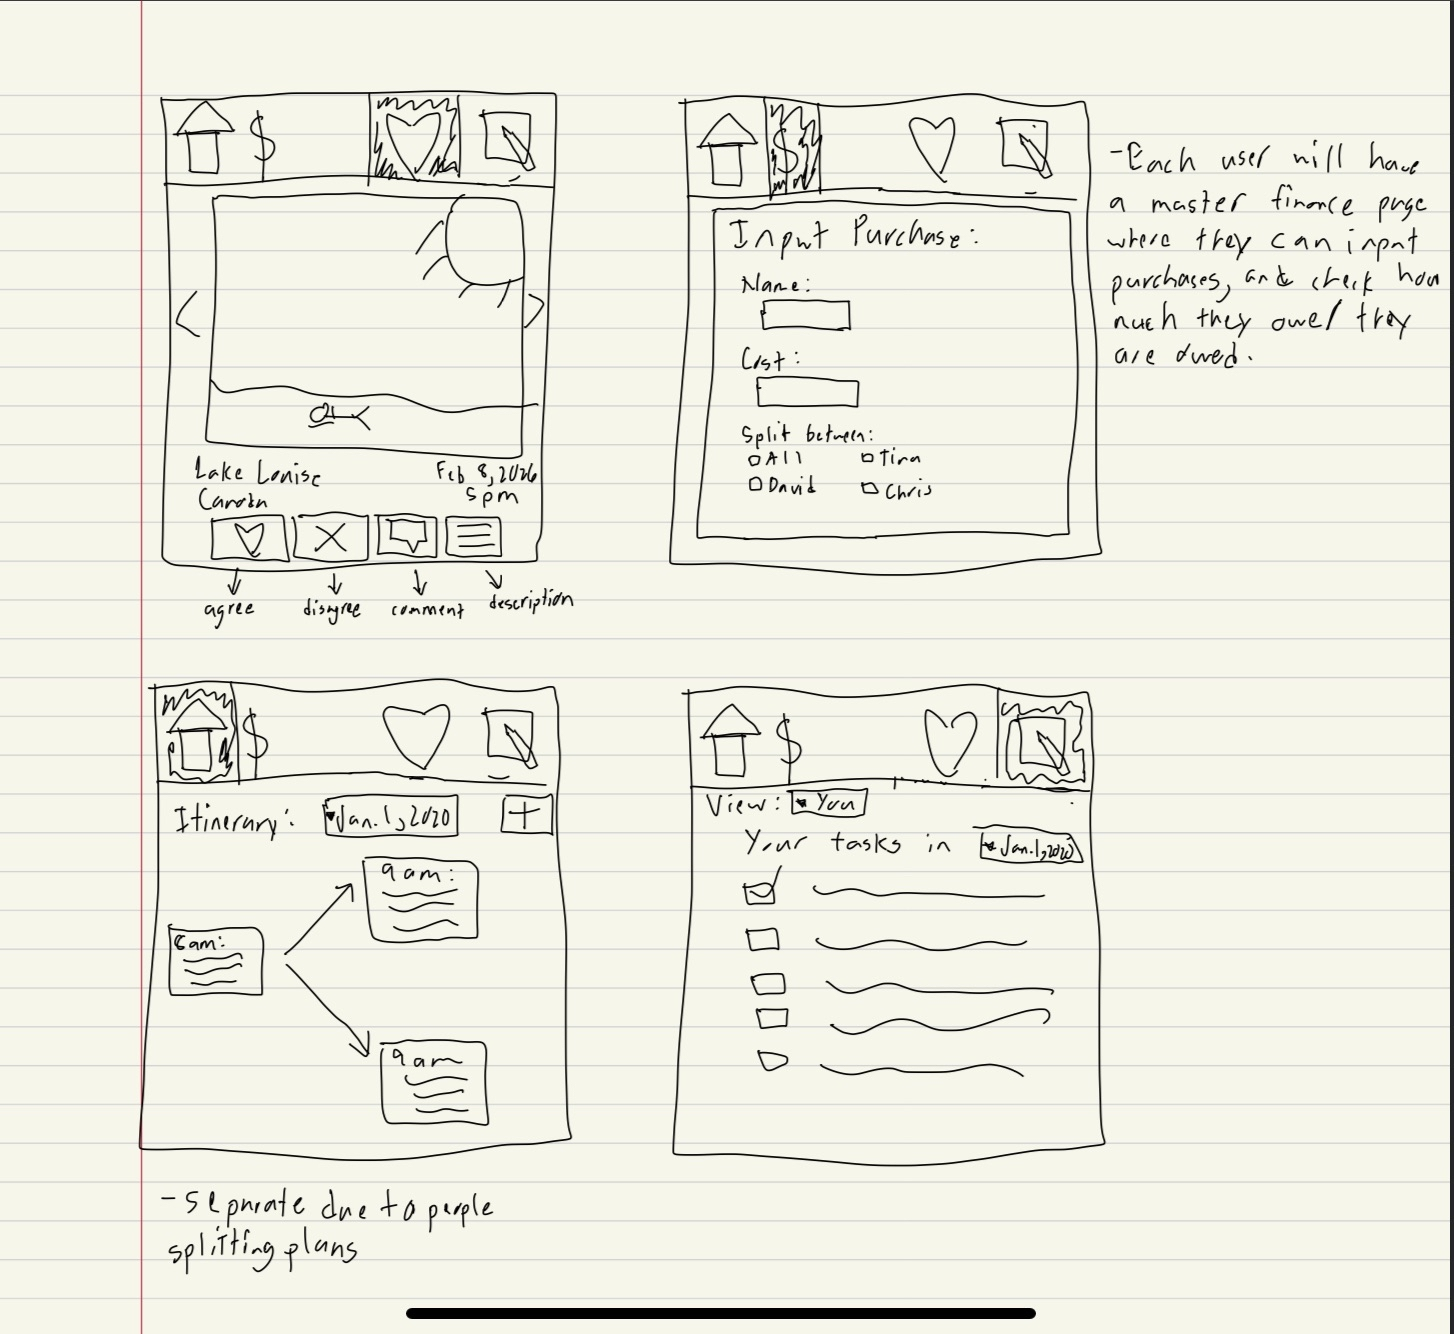
\includegraphics[width=\linewidth]{IMG_0248.png}
    \caption{Design 1}
    \label{fig:design1}
\end{figure}

%\subsection{Design 2}

\subsection{Design 2}
\label{app:design2}
\begin{figure}[H]
    \centering
    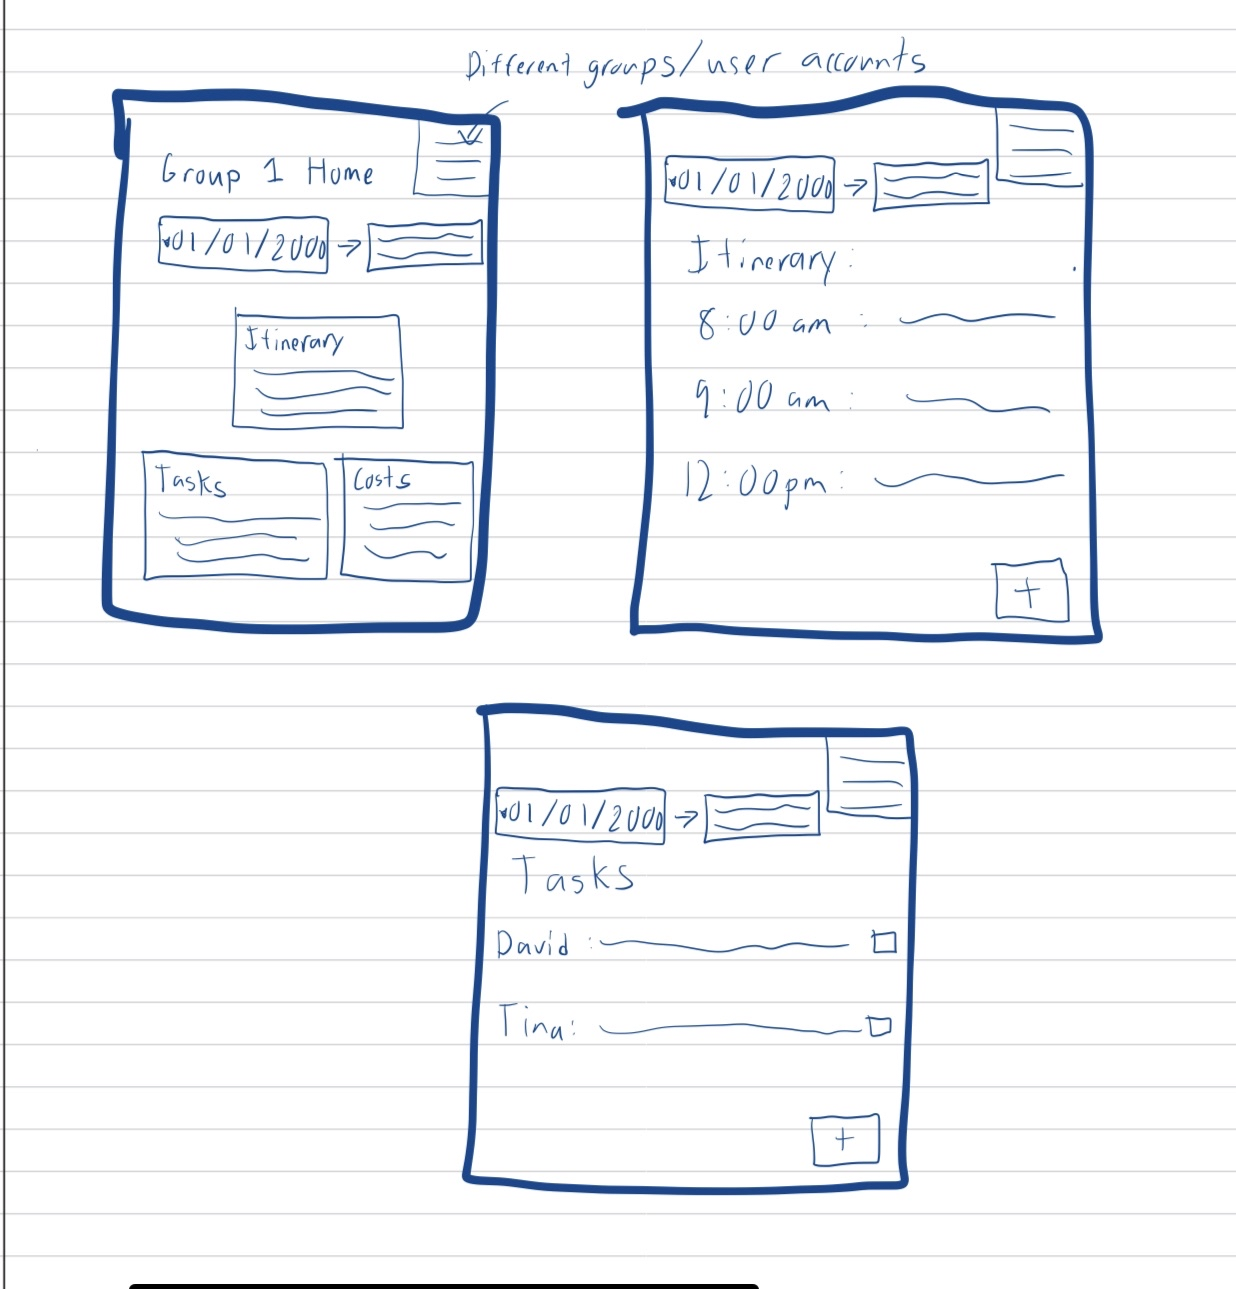
\includegraphics[width=\linewidth]{IMG_0249.png}
    \caption{Design 2}
    \label{fig:design2}
\end{figure}

%\subsection{Design 3}

\subsection{Design 3}
\label{app:design3}
\begin{figure}[H]
    \centering
    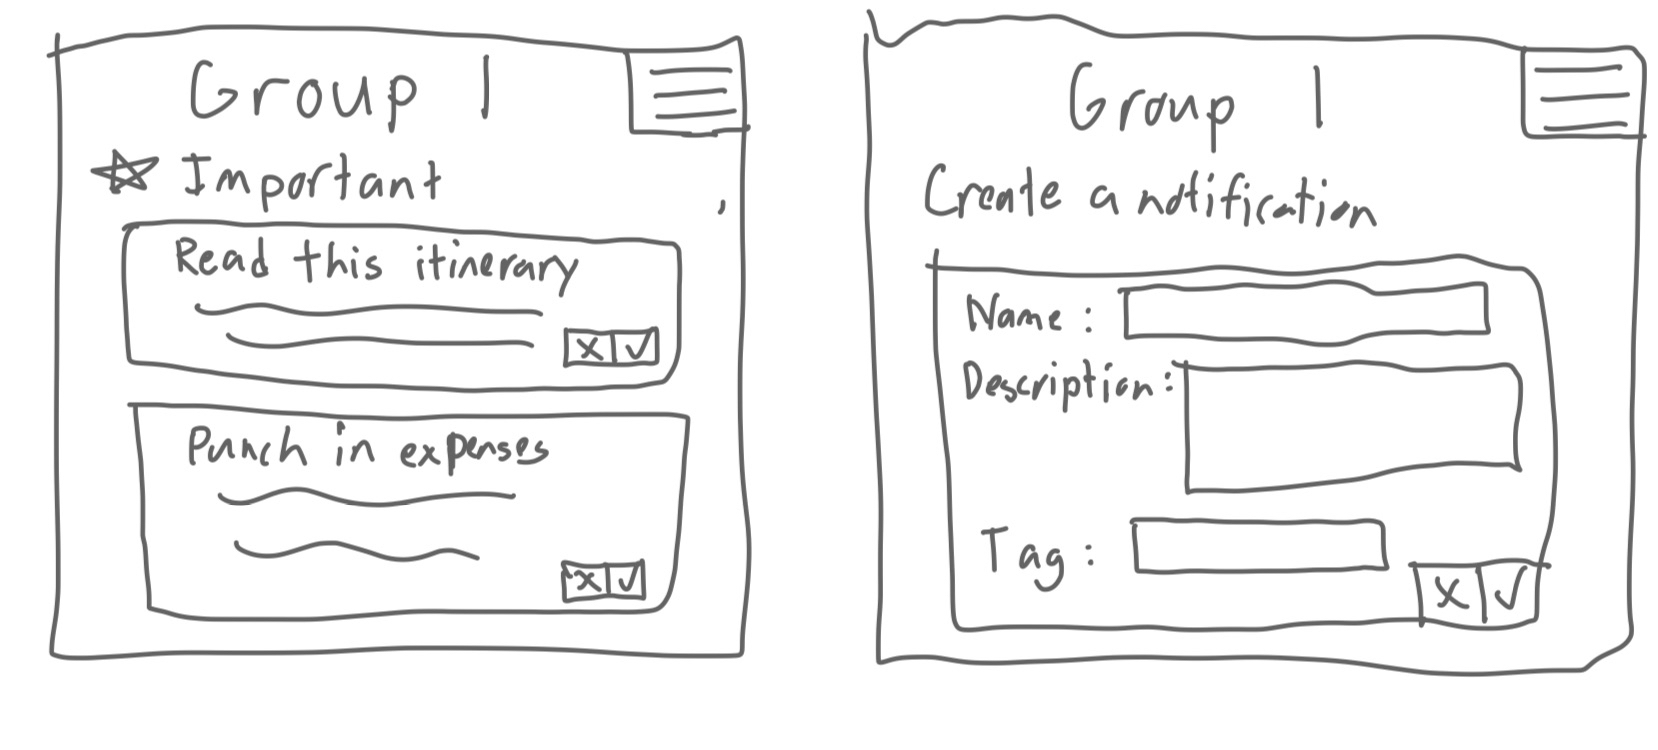
\includegraphics[width=\linewidth]{IMG_0250.png}
    \caption{Design 3}
    \label{fig:design3}
\end{figure}

%\subsection{Design 4}
\subsection{Design 4}
\label{app:design4}
\begin{figure}[H]
    \centering
    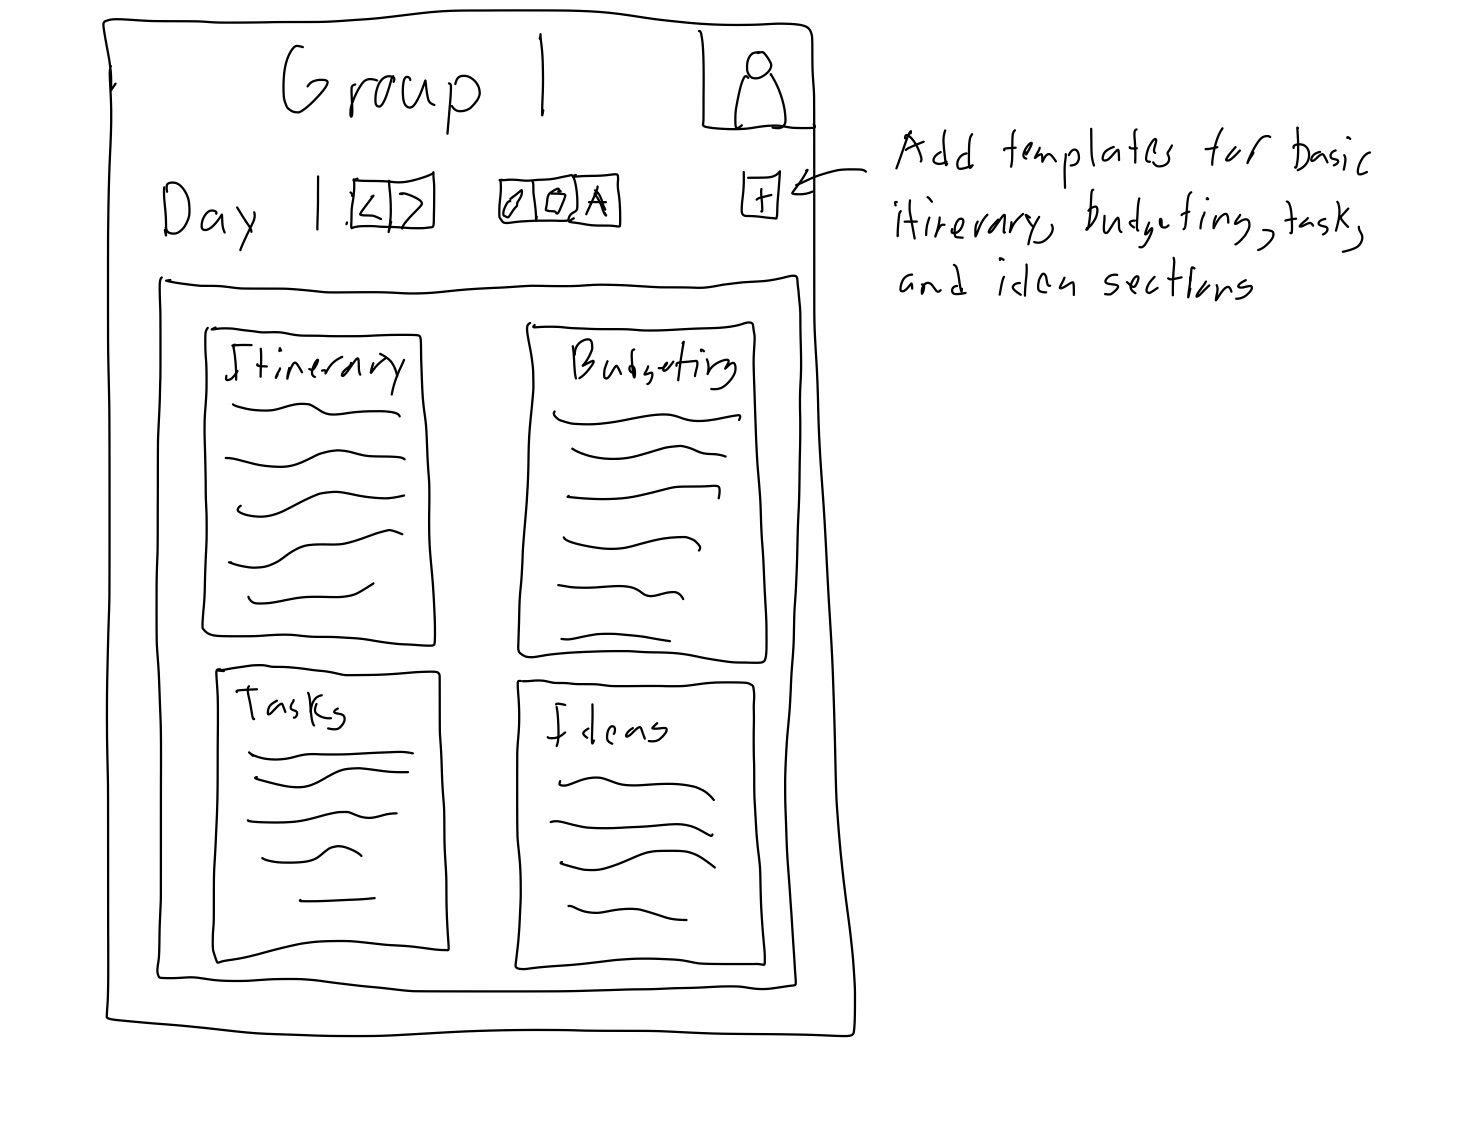
\includegraphics[width=\linewidth]{IMG_0252.png}
    \caption{Design 4}
    \label{fig:design4}
\end{figure}

\label{app:design5}
\subsection{Design 5}
\begin{figure}[H]
    \centering
    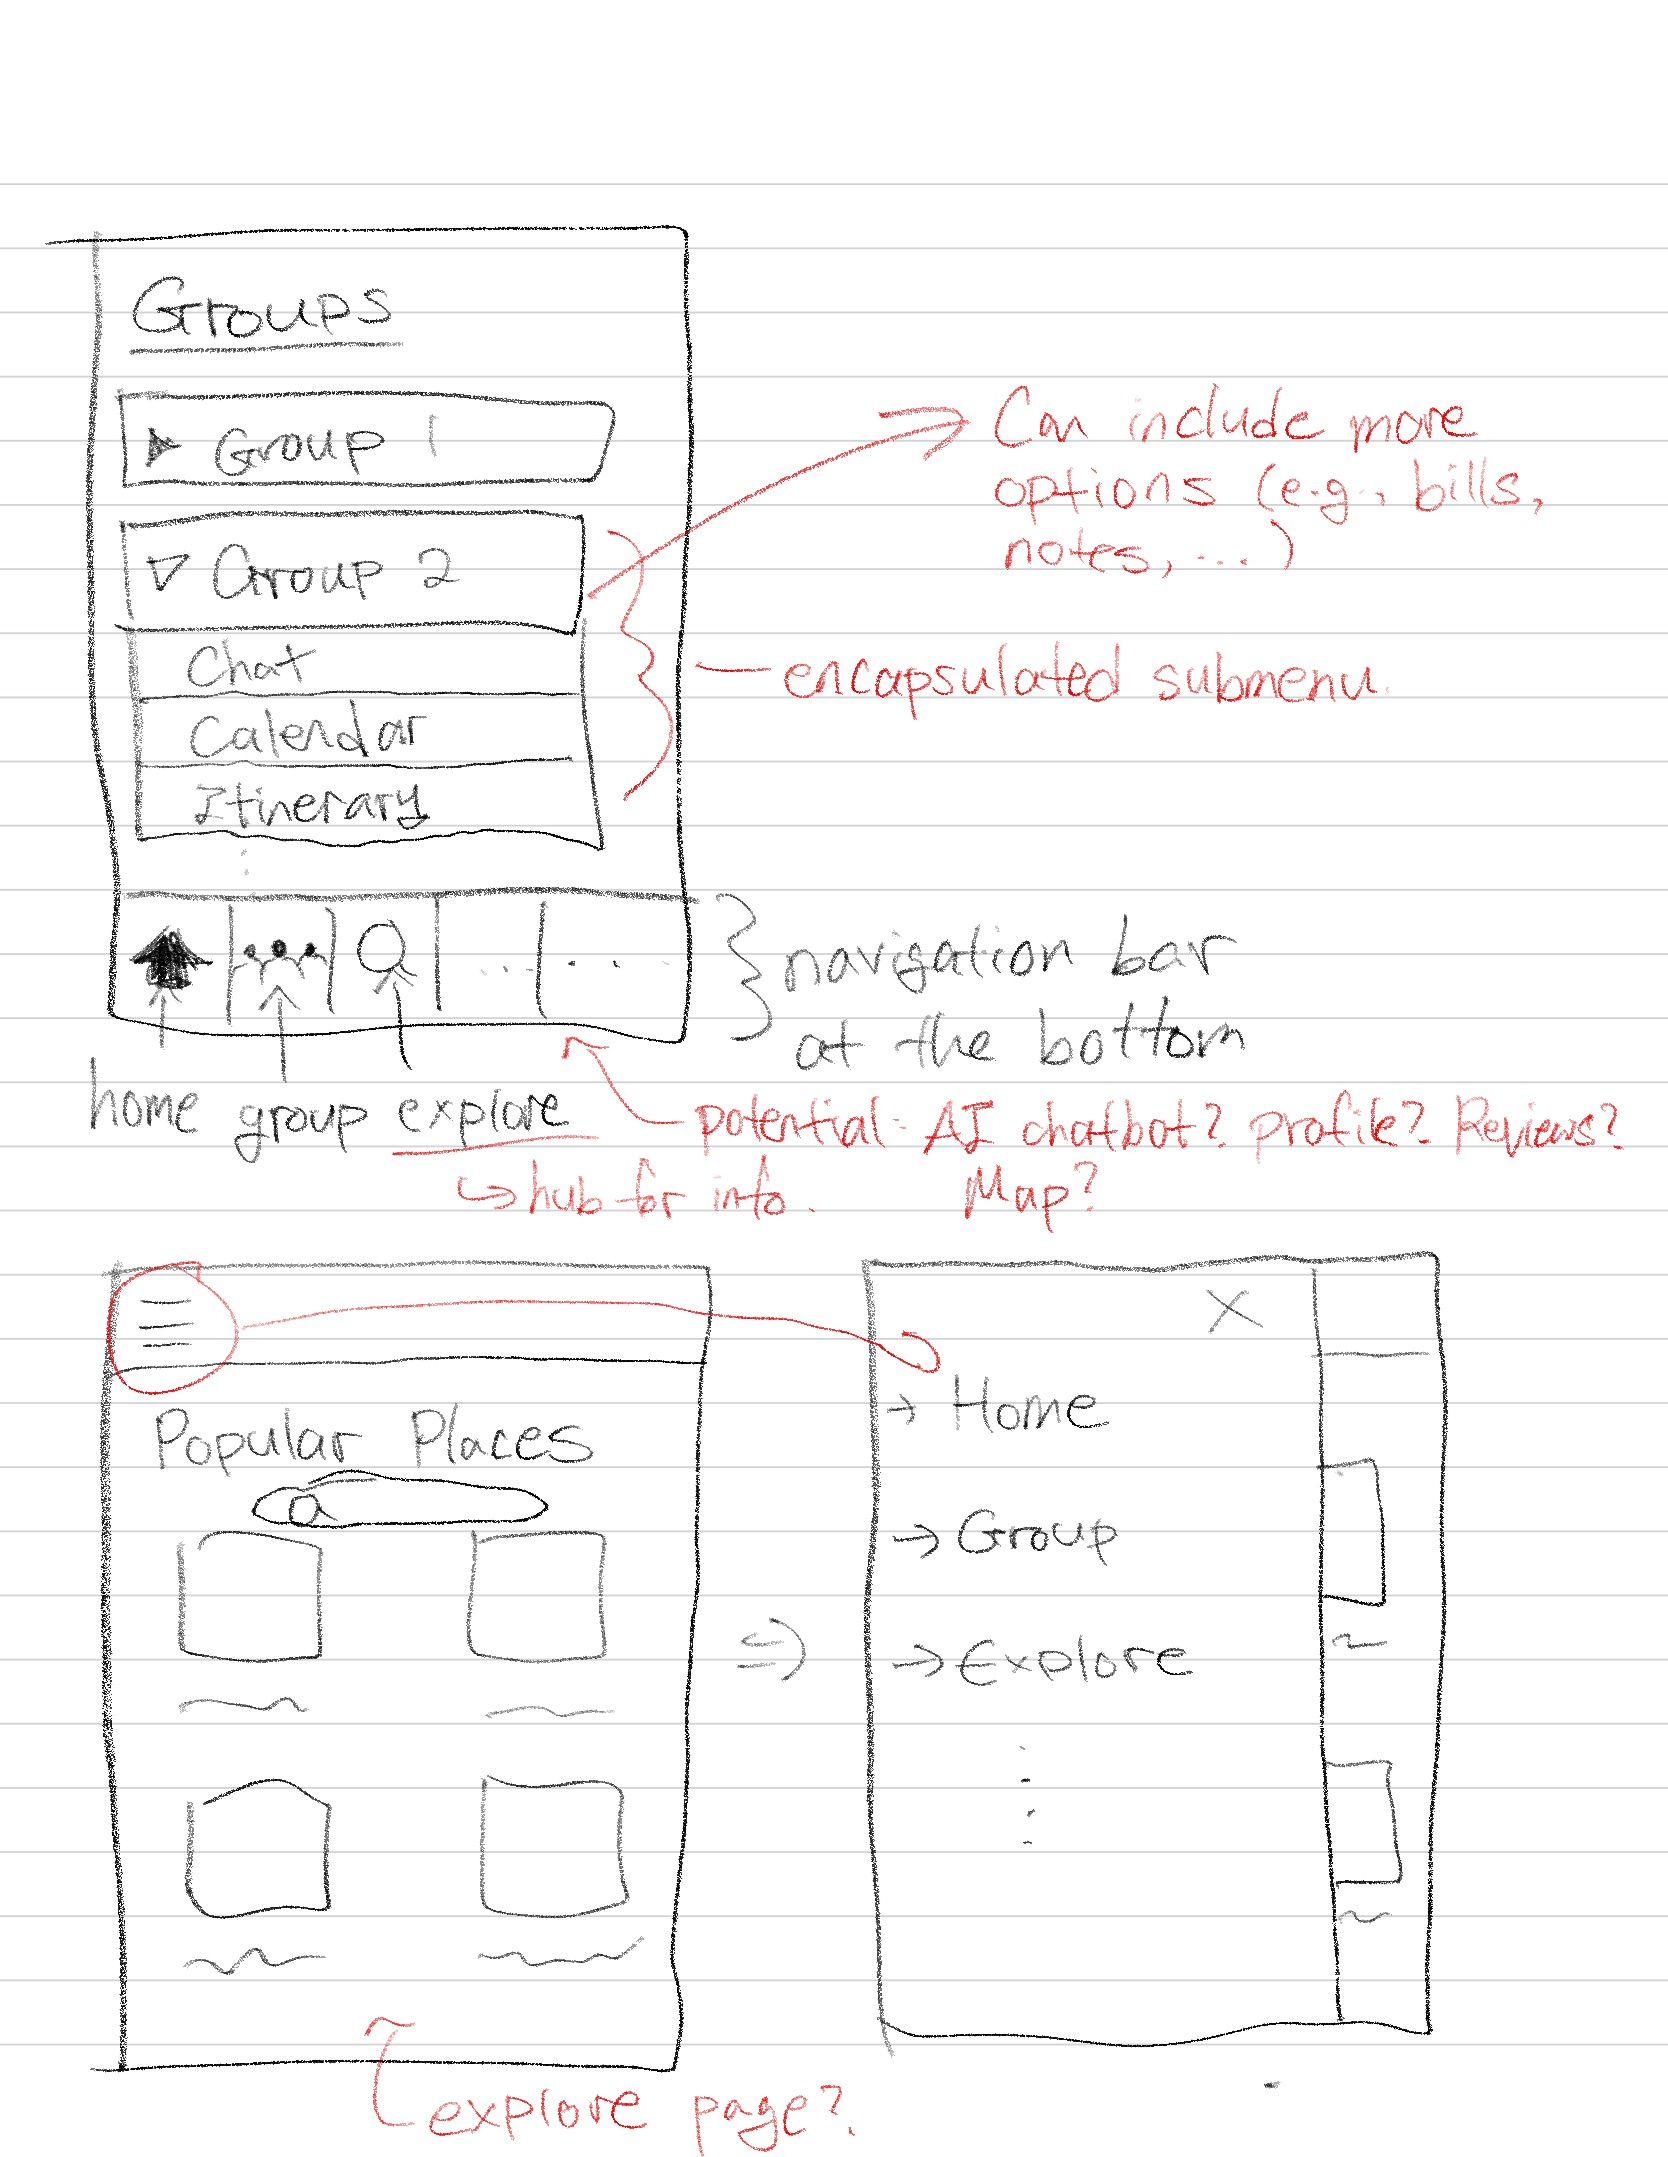
\includegraphics[width=\linewidth]{Project-1.jpeg}
    \caption{Design 5}
    \label{fig:design5}
\end{figure}

\label{app:design6}
\subsection{Design 6}
\begin{figure}[H]
    \centering
    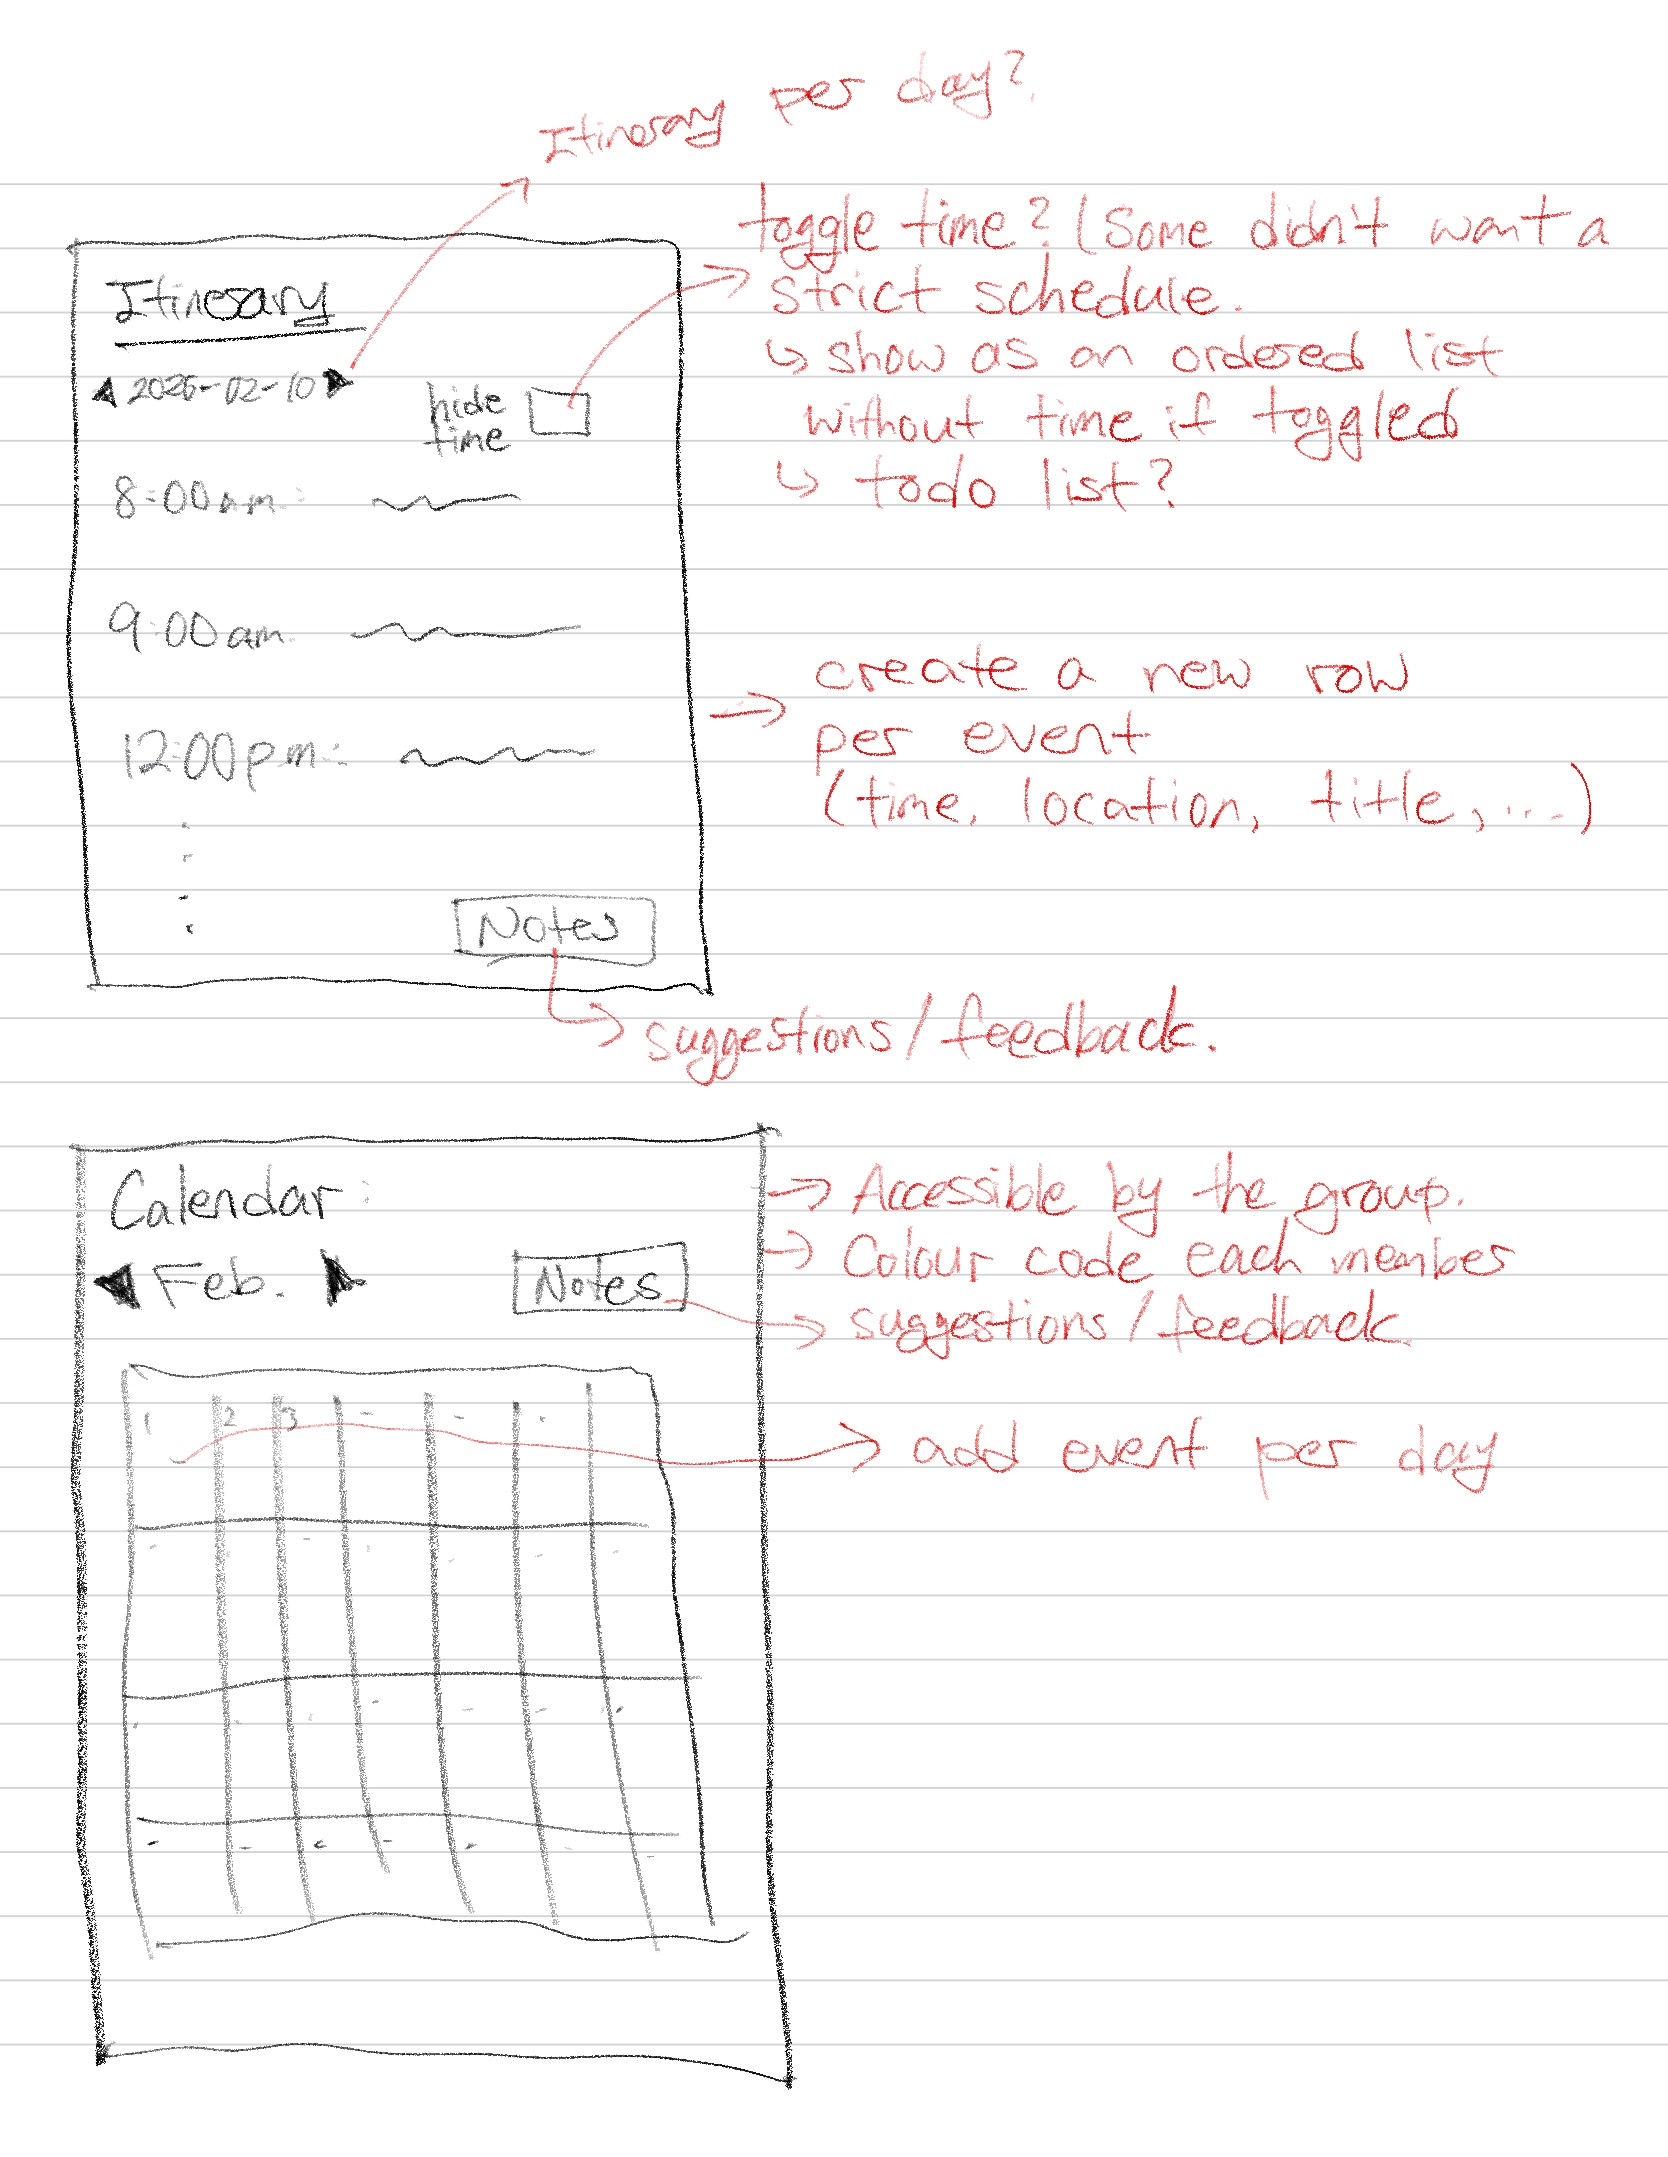
\includegraphics[width=\linewidth]{Project-2.jpeg}
    \caption{Design 6}
    \label{fig:design6}
\end{figure}

\label{app:design7}
\subsection{Design 7}
\begin{figure}[H]
    \centering
    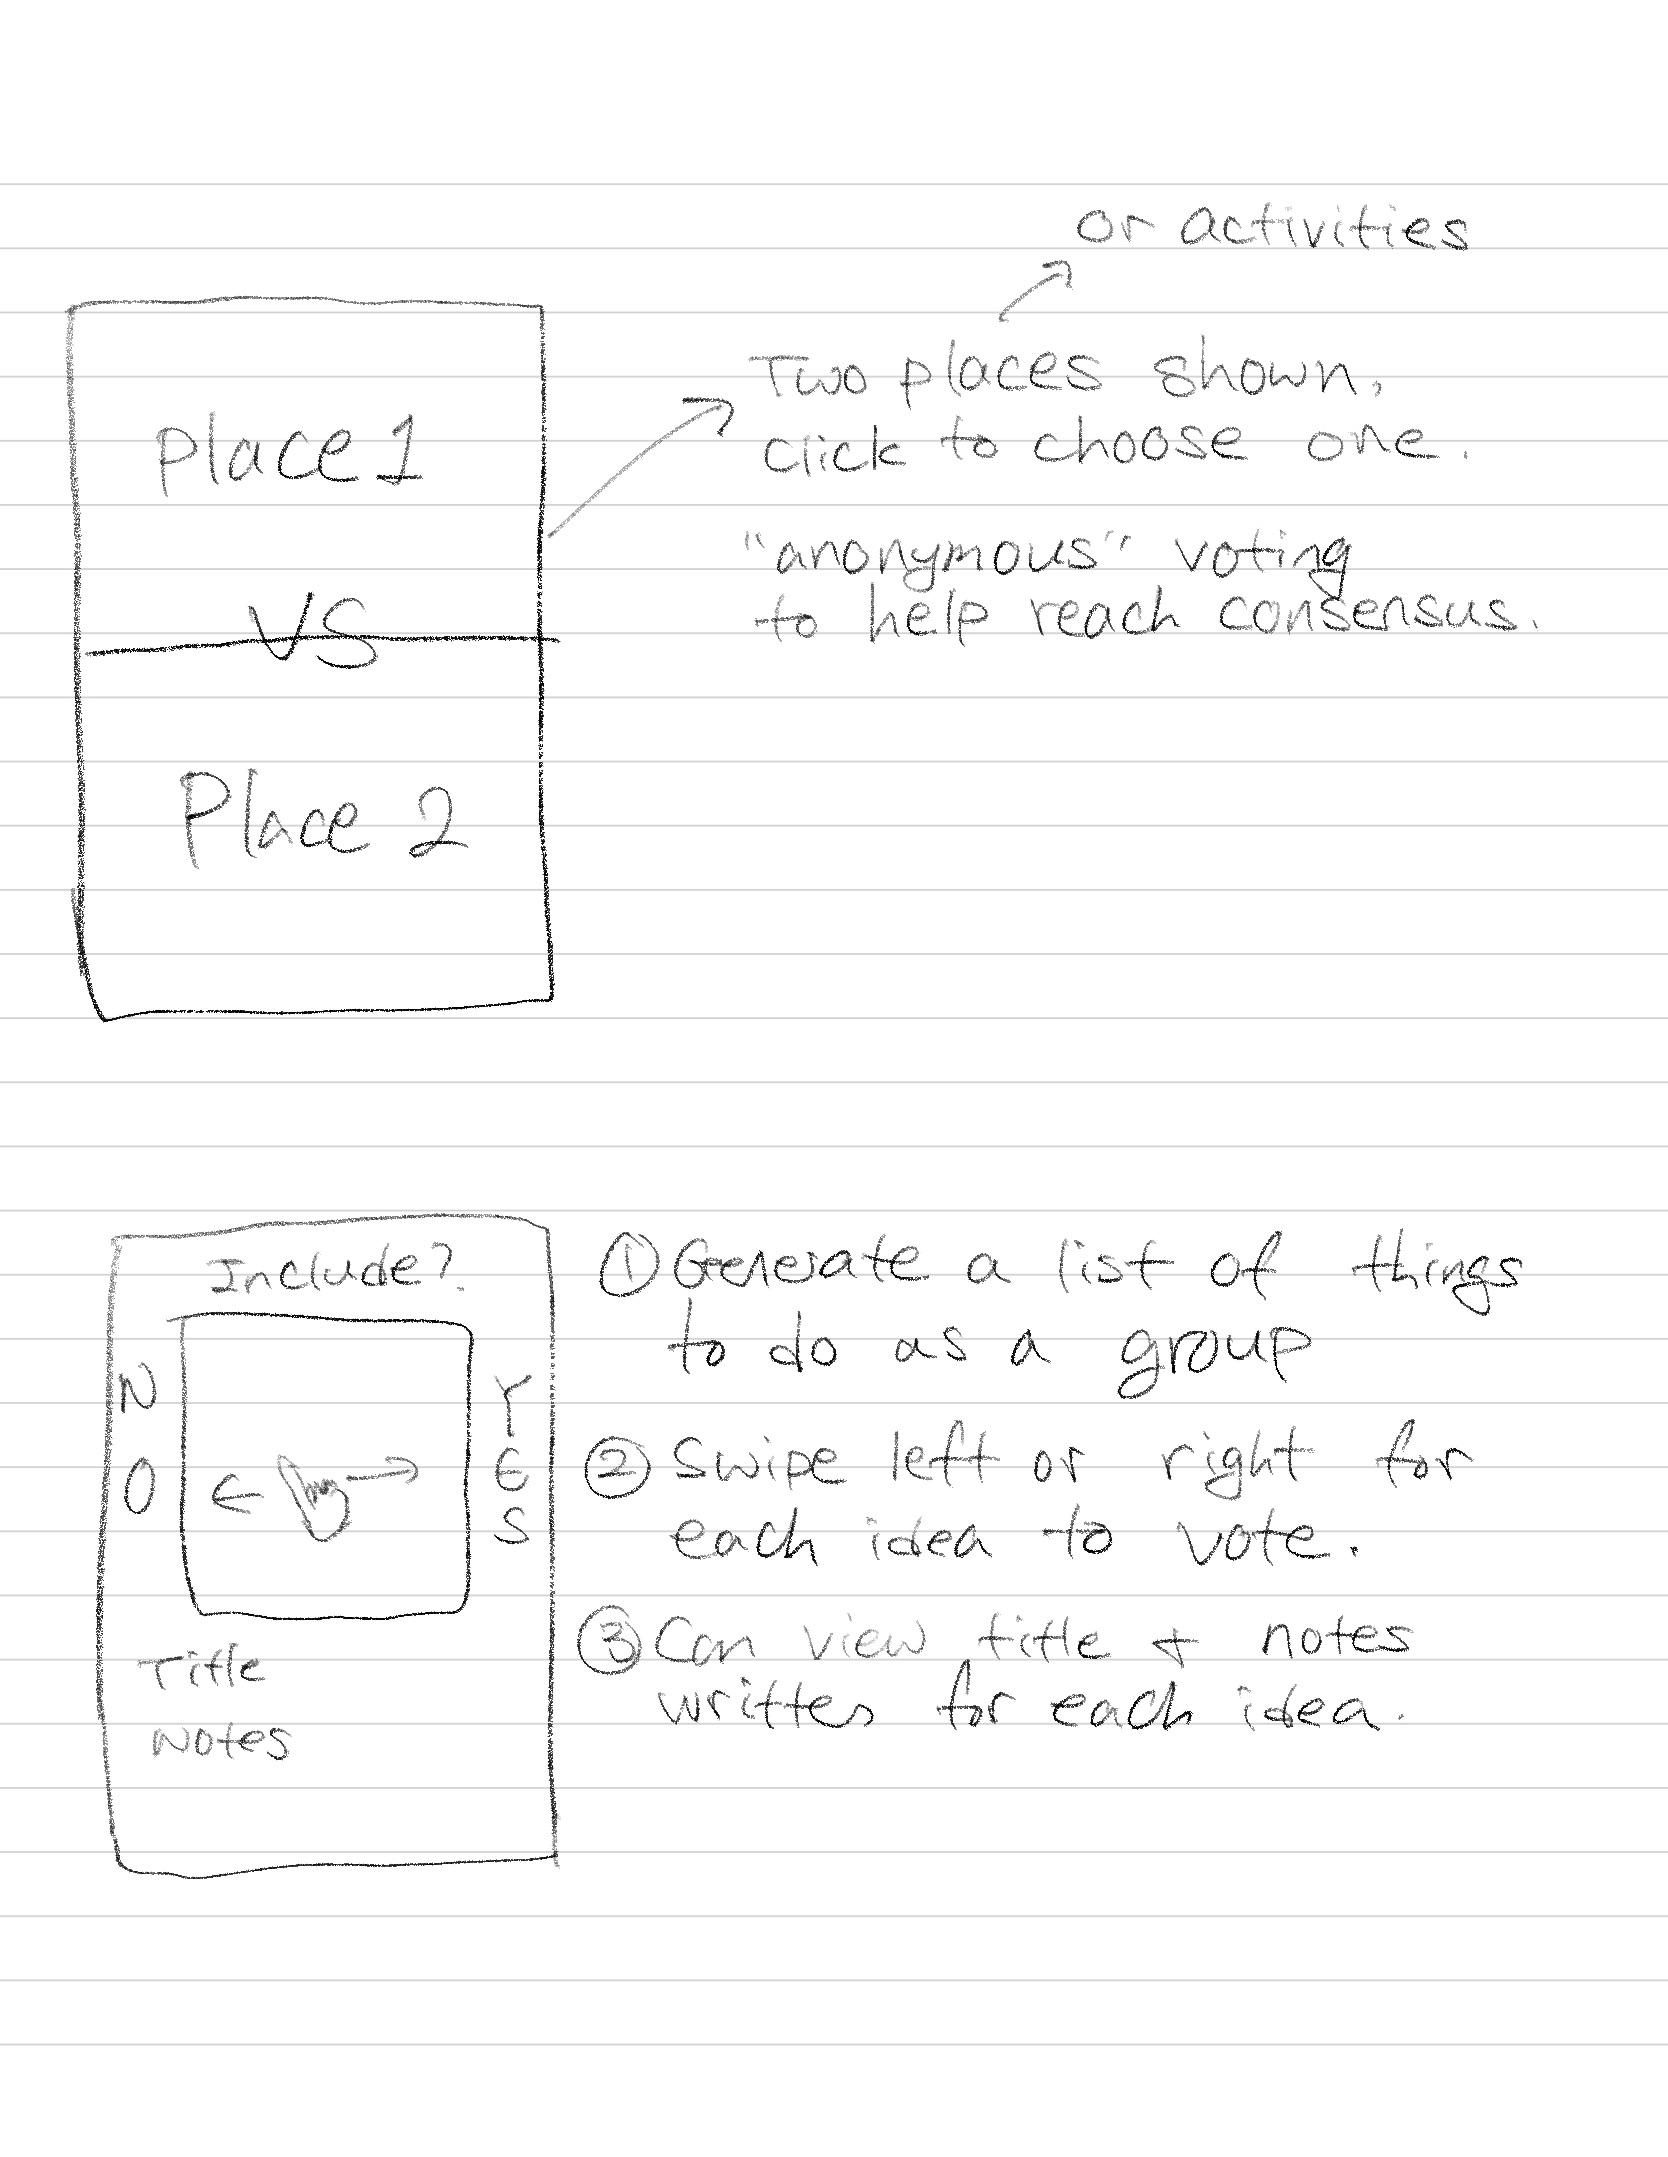
\includegraphics[width=\linewidth]{Project-3.jpeg}
    \caption{Design 7}
    \label{fig:design7}
\end{figure}

\label{app:design8}
\subsection{Design 8}
\begin{figure}[H]
    \centering
    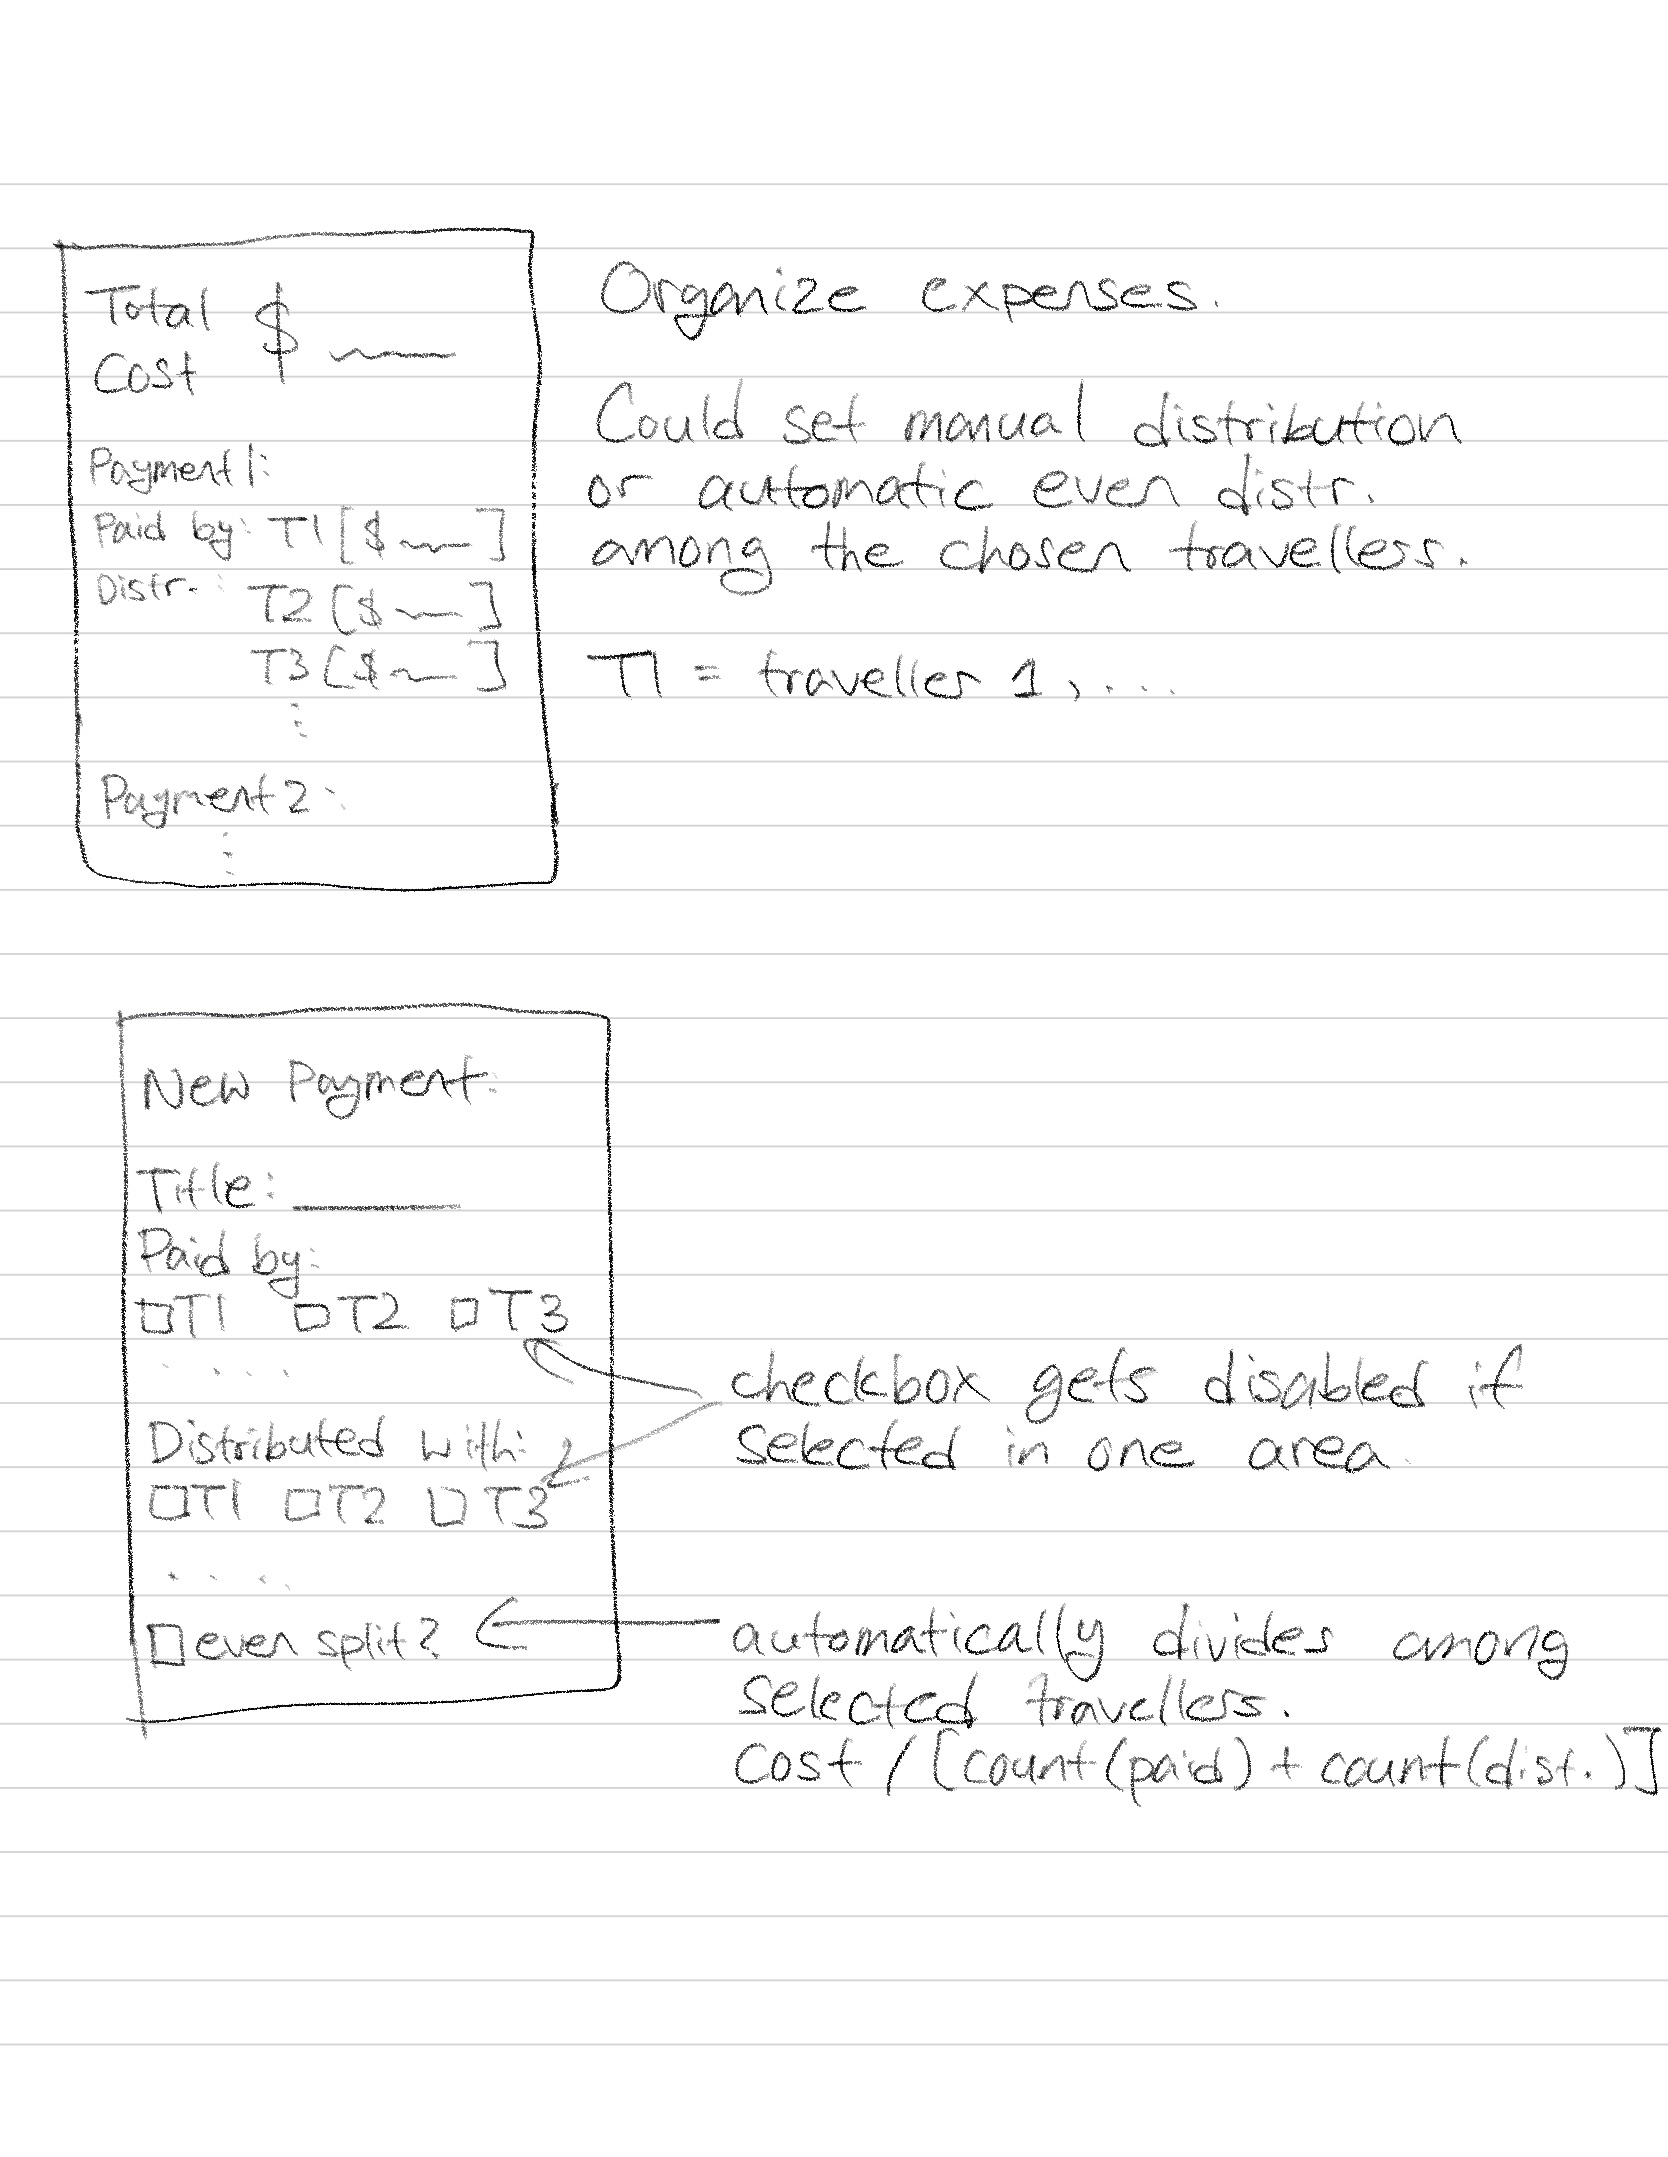
\includegraphics[width=\linewidth]{Project-4.jpeg}
    \caption{Design 8}
    \label{fig:design8}
\end{figure}

\label{app:design9}
\subsection{Design 9}
\begin{figure}[H]
    \centering
    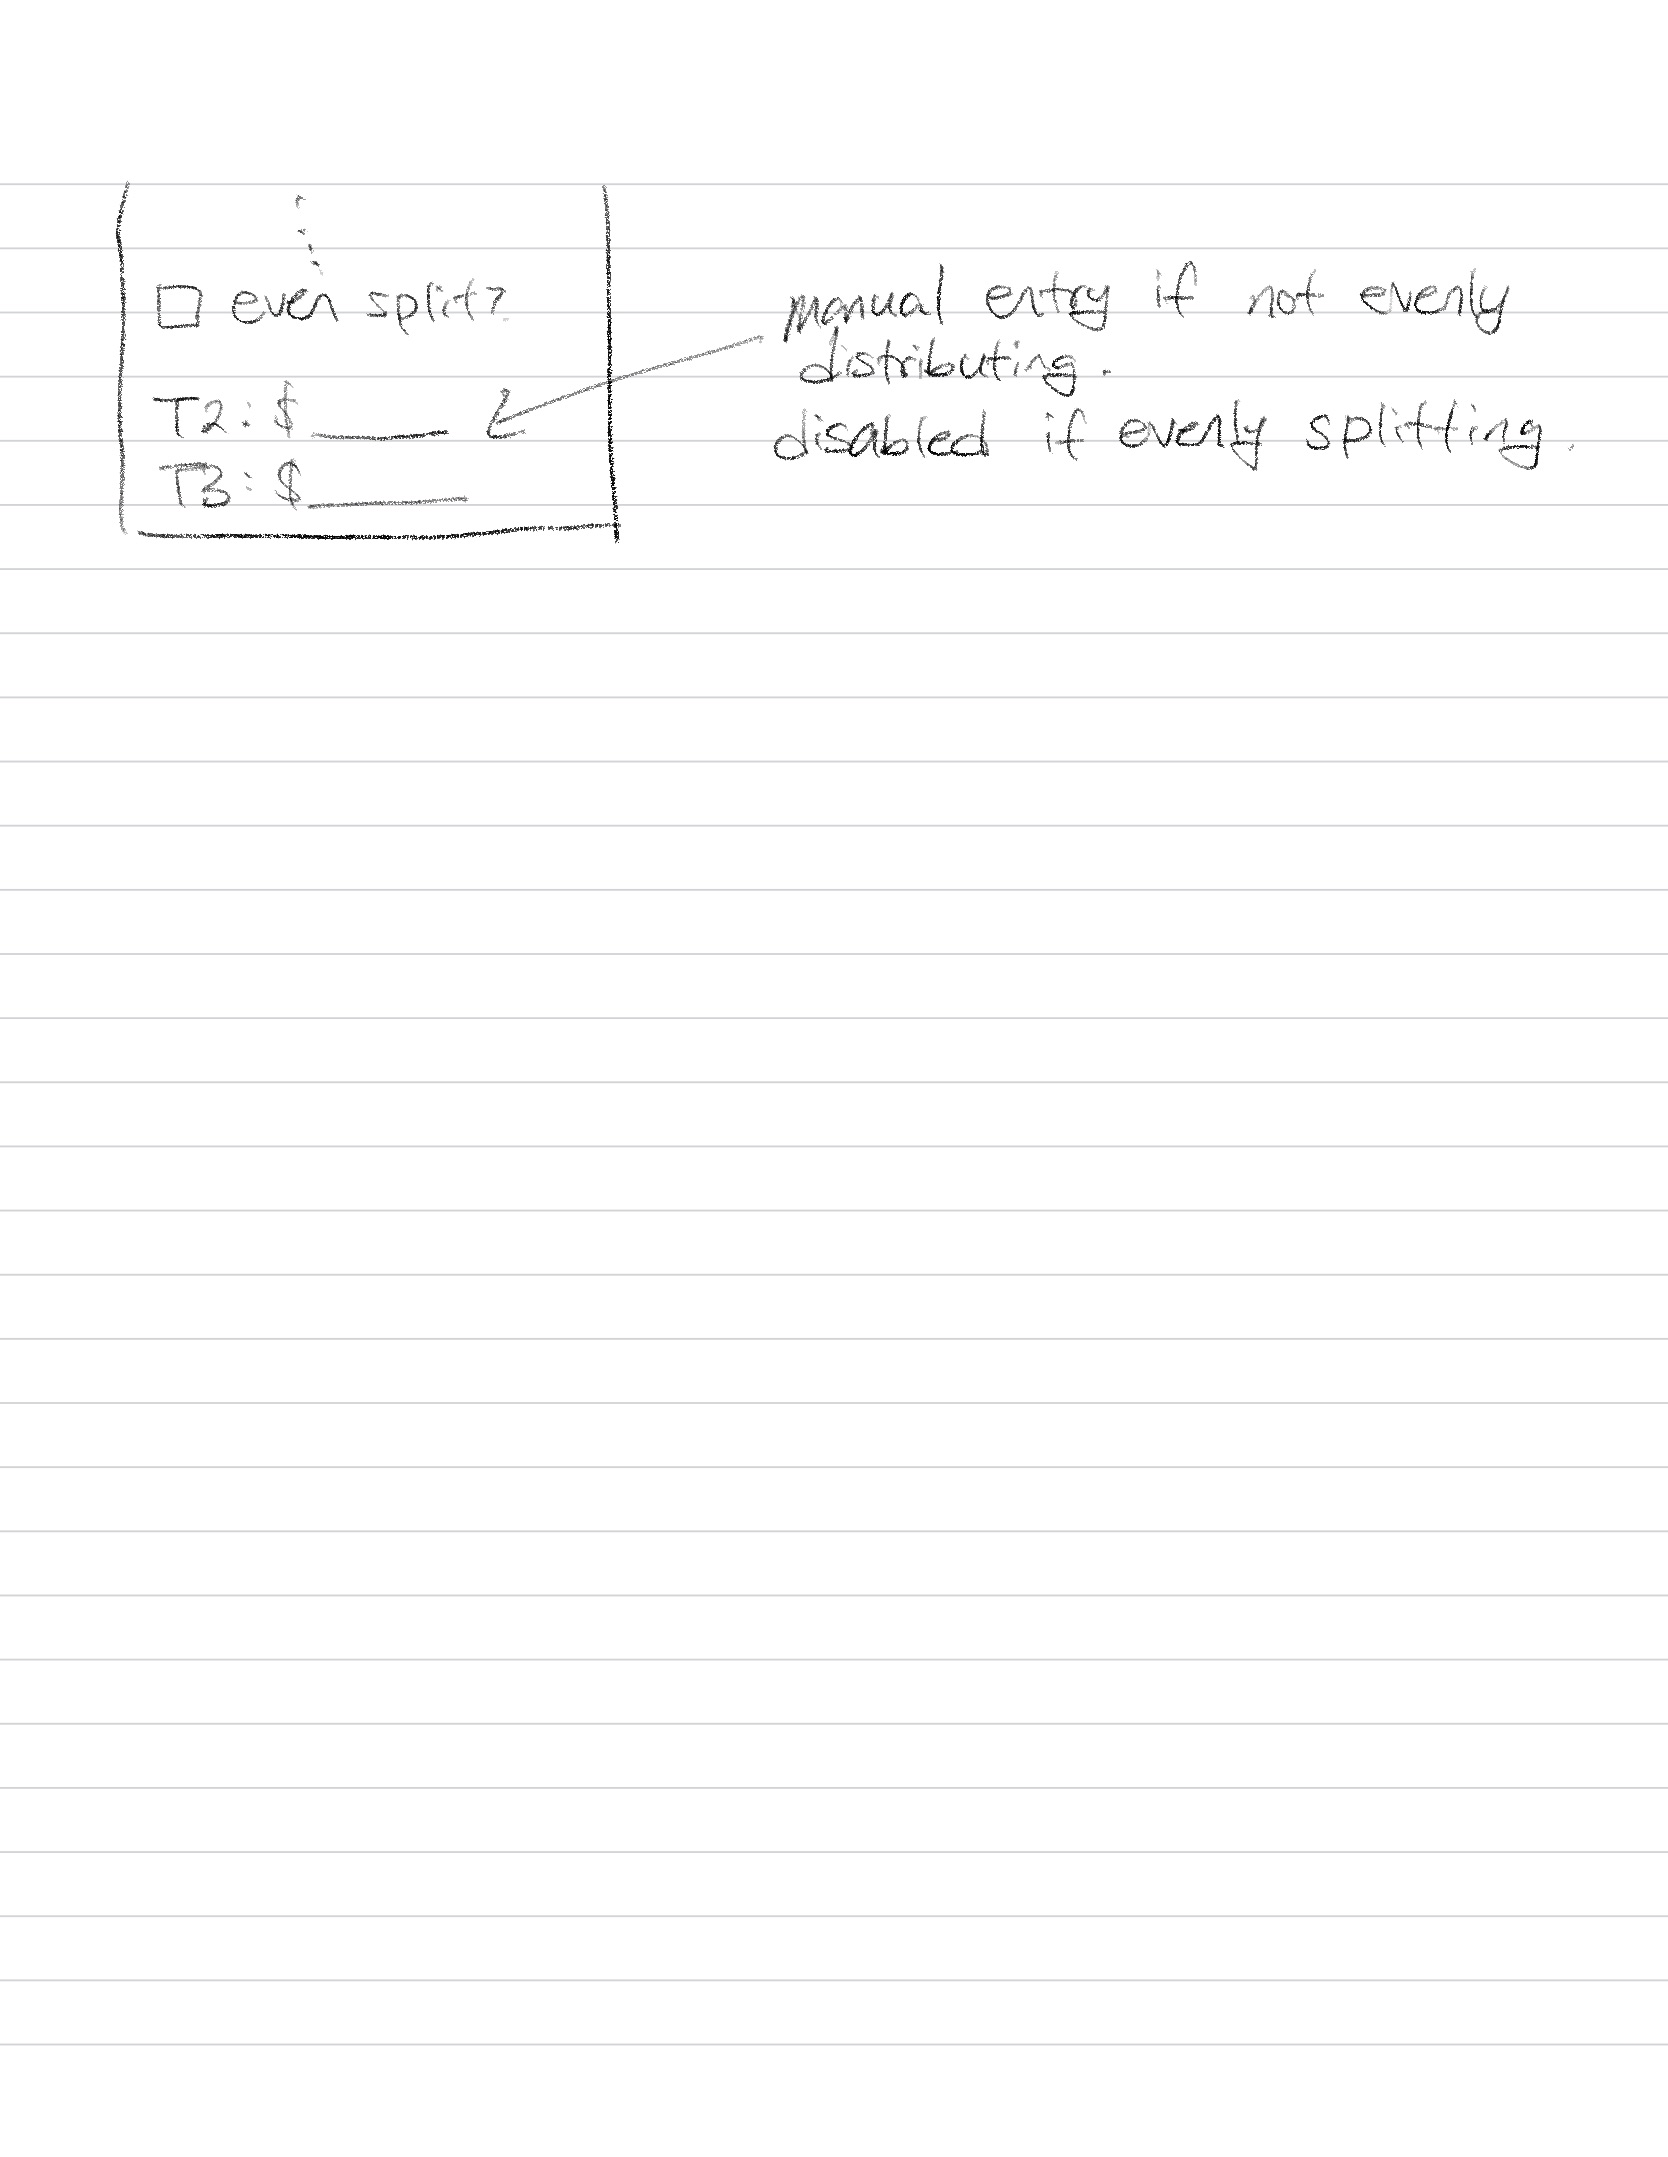
\includegraphics[width=\linewidth]{Project-5.jpeg}
    \caption{Design 9}
    \label{fig:design9}
\end{figure}

\newpage
\section{Additional Materials}
\subsection{MyMaps - Observation}
\begin{figure}[H]
    \centering
    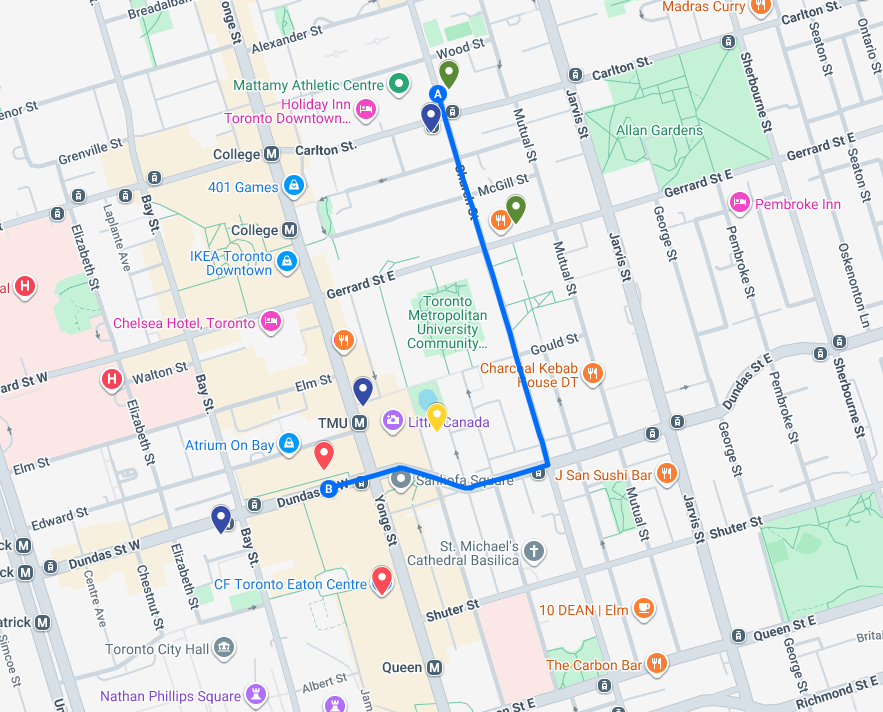
\includegraphics[width=\linewidth]{mymap1.png}
    \caption{Google My Map Example 1}
    \label{fig:design1}
\end{figure}

\begin{figure}[H]
    \centering
    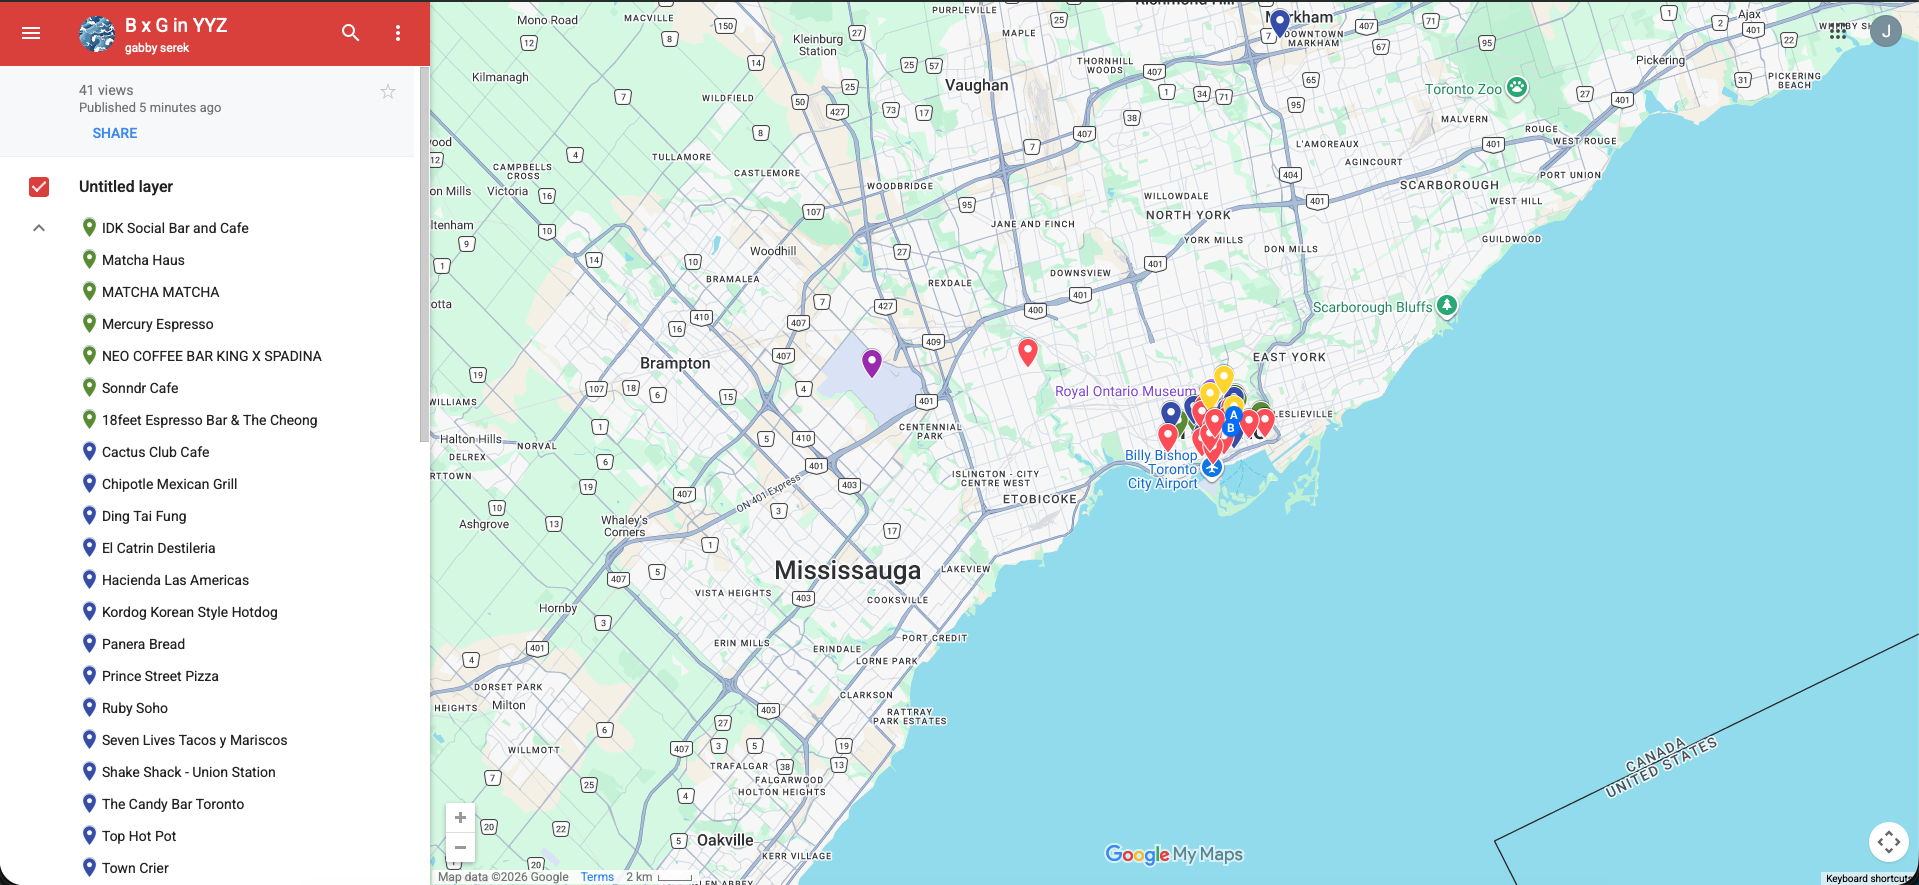
\includegraphics[width=\linewidth]{mymap2.png}
    \caption{Google My Map Example 2}
    \label{fig:MyMap2}
\end{figure}

\begin{figure}[H]
    \centering
    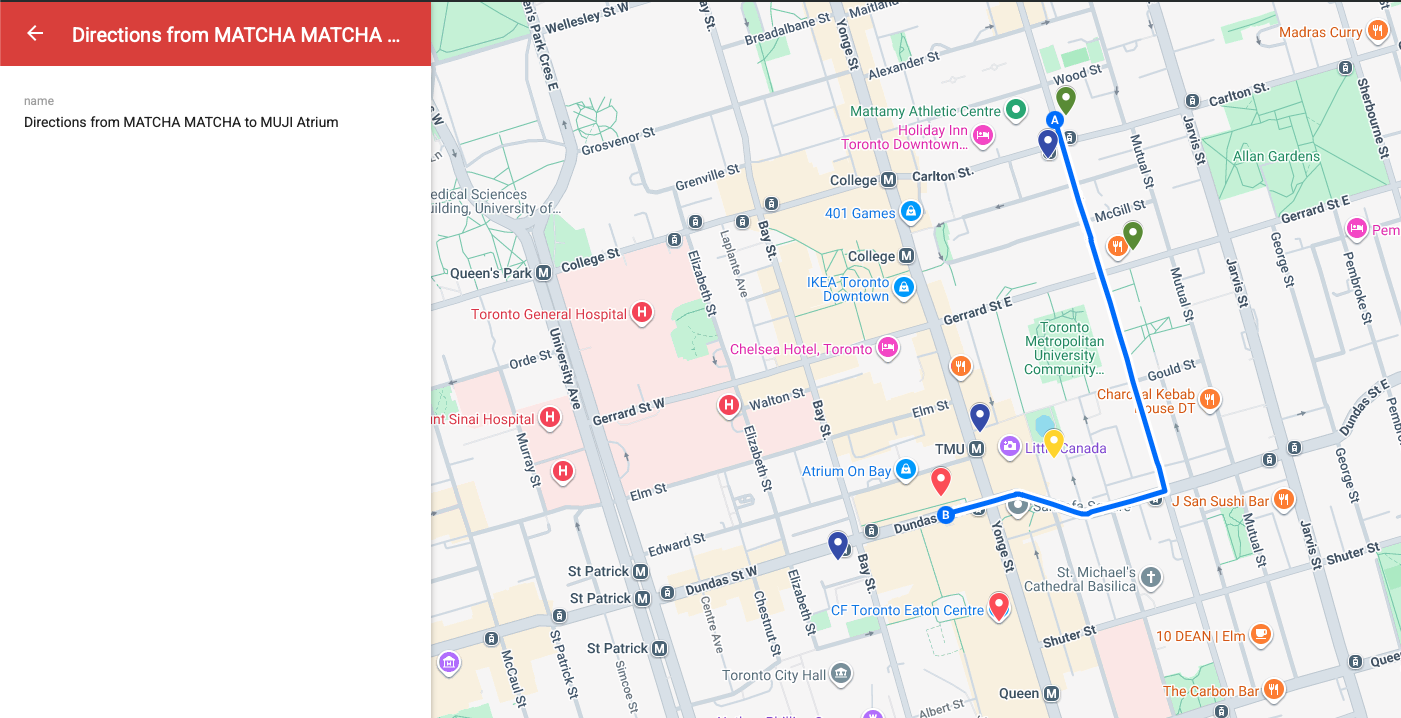
\includegraphics[width=\linewidth]{mymap4.png}
    \caption{Google My Map Example 3}
    \label{fig:MyMap3}
\end{figure}

\begin{figure}[H]
    \centering
    
    \begin{minipage}{0.48\linewidth}
        \centering
        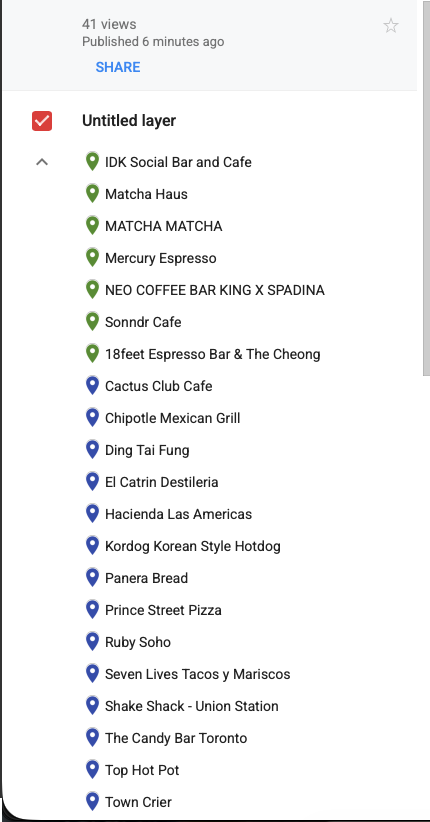
\includegraphics[width=\linewidth]{mymap3.png}
        \caption{Google My Map Example 4}
        \label{fig:MyMap4}
    \end{minipage}
    \hfill
    \begin{minipage}{0.48\linewidth}
        \centering
        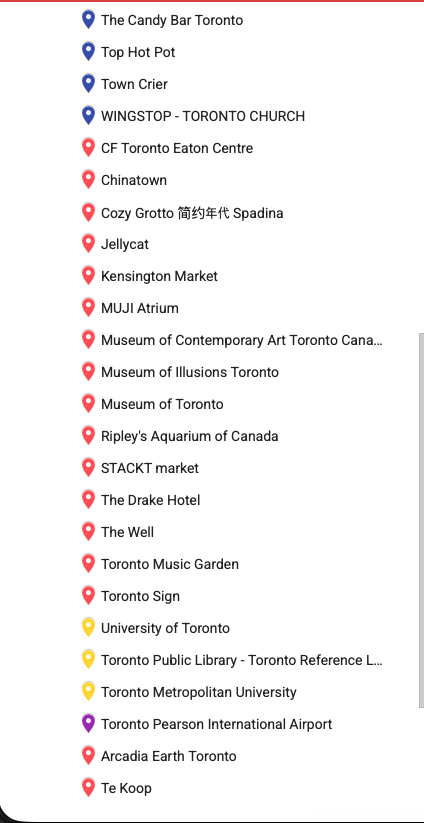
\includegraphics[width=\linewidth]{mymap5.png}
        \caption{Google My Map Example 5}
        \label{fig:MyMap5}
    \end{minipage}
    
\end{figure}
\end{document}
